% !TEX program = xelatex
% ==============================================================================
% KHÓA LUẬN TỐT NGHIỆP ĐẠI HỌC - TRƯỜNG ĐH CÔNG NGHỆ THÔNG TIN (ĐHQG-HCM)
% Trình biên dịch: XeLaTeX | Font: Times New Roman (UTF-8)
% Kế thừa và chuẩn hóa theo mẫu quy định của Bộ GD&ĐT và Trường ĐH CNTT
% ==============================================================================

\documentclass[13pt,a4paper,oneside]{report}

% ------------------------------------------------------------------------------
% 1. CẤU HÌNH FONT VÀ TIẾNG VIỆT
% ------------------------------------------------------------------------------
\usepackage{fontspec}          % Nạp font OpenType/TrueType cho XeLaTeX
\setmainfont{Times New Roman}  % Font Times New Roman chuẩn mực

\usepackage[vietnamese]{babel} % Tự động Việt hóa tiêu đề: Chương, Mục lục, Hình, Bảng...

% ------------------------------------------------------------------------------
% 2. CĂN LỀ TRANG IN (CHUẨN QUY ĐỊNH PHỤ LỤC 2 TRƯỜNG ĐH CNTT)
% Quy định: Lề trên 3cm (30mm), Lề dưới 3.5cm (35mm), Lề trái 3.5cm (35mm), Lề phải 2cm (20mm)
% ------------------------------------------------------------------------------
\usepackage{geometry}
\geometry{
    a4paper,
    top=30mm,
    bottom=35mm,
    left=35mm,
    right=20mm
}

% ------------------------------------------------------------------------------
% 3. GIÃN DÒNG VÀ ĐỊNH DẠNG ĐOẠN VĂN
% ------------------------------------------------------------------------------
\usepackage{setspace}
\onehalfspacing             % Giãn dòng 1.5 dòng theo quy định chuẩn

\usepackage{indentfirst}    % Tự động thụt đầu dòng cả đoạn văn đầu tiên sau tiêu đề
\setlength{\parindent}{1cm} % Thụt lề đầu dòng 1cm
\setlength{\parskip}{6pt}   % Khoảng cách giữa các đoạn văn 6pt

% ------------------------------------------------------------------------------
% 4. CÁC GÓI TIỆN ÍCH HỖ TRỢ (TOÁN, BẢNG BIỂU, HÌNH ẢNH, VIỀN BÌA TIKZ)
% ------------------------------------------------------------------------------
\usepackage{amsmath, amsfonts, amssymb}
\usepackage{graphicx}
\usepackage{booktabs}
\usepackage{array}
\usepackage{tikz}
\usetikzlibrary{calc}
\usepackage{caption}
\captionsetup{
    font=small,
    labelfont=bf,
    labelsep=colon,
    justification=centering
}

\usepackage[unicode]{hyperref}
\hypersetup{
    colorlinks=true,
    linkcolor=black,        % Màu đen chuẩn mực cho liên kết nội bộ
    citecolor=blue,         % Màu xanh lam cho trích dẫn tài liệu
    urlcolor=blue           % Màu xanh lam cho URL
}

% ==============================================================================
% BẮT ĐẦU TÀI LIỆU
% ==============================================================================
\begin{document}

% ------------------------------------------------------------------------------
% PHẦN TRANG BÌA VÀ THỦ TỤC ĐẦU BÁO CÁO (KHÔNG ĐÁNH SỐ TRANG THEO PHỤ LỤC 2)
% ------------------------------------------------------------------------------
\pagestyle{empty}
% Trang bìa chính thức Khóa luận tốt nghiệp UIT (Bìa ngoài)
\begin{titlepage}
    % Khung viền đôi chuẩn học thuật UIT
    \begin{tikzpicture}[remember picture, overlay]
        \draw[line width = 2pt] 
            ($(current page.north west) + (2.5cm,-1.5cm)$) 
            rectangle 
            ($(current page.south east) + (-1.5cm,1.5cm)$);
        \draw[line width = 0.8pt] 
            ($(current page.north west) + (2.6cm,-1.6cm)$) 
            rectangle 
            ($(current page.south east) + (-1.4cm,1.4cm)$);
    \end{tikzpicture}
    
    \centering
    {\fontsize{15pt}{18pt}\selectfont \textbf{ĐẠI HỌC QUỐC GIA THÀNH PHỐ HỒ CHÍ MINH}}\\[0.2cm]
    {\fontsize{16pt}{20pt}\selectfont \textbf{TRƯỜNG ĐẠI HỌC CÔNG NGHỆ THÔNG TIN}}\\[0.2cm]
    {\fontsize{16pt}{20pt}\selectfont \textbf{KHOA KHOA HỌC MÁY TÍNH}}\\[0.3cm]
    {\fontsize{10pt}{12pt}\selectfont —————————— ❖ ——————————}\\[0.6cm]

    % Logo trường Đại học Công nghệ Thông tin
    
\includegraphics[width=3.2cm]{figures/logo_uit.jpeg}\\[1.0cm]

    {\fontsize{14pt}{18pt}\selectfont \textbf{ĐÀO PHƯỚC THỊNH}}\\[0.15cm]
    {\fontsize{14pt}{18pt}\selectfont \textbf{HÀ QUANG ĐẠT}}\\[1.0cm]

    {\fontsize{16pt}{20pt}\selectfont \textbf{KHÓA LUẬN TỐT NGHIỆP}}\\[0.5cm]

    % Tên đề tài khóa luận (Tiếng Việt & Tiếng Anh)
    \begin{minipage}{0.92\textwidth}
        \centering
        {\fontsize{18pt}{22pt}\selectfont \textbf{NGHIÊN CỨU PHƯƠNG PHÁP TOOL CALLING DỰA TRÊN TRUY HỒI NGỮ NGHĨA VÀ TRÍCH XUẤT THAM SỐ THEO TOOL SCHEMA}}\\[0.5cm]
        {\fontsize{16pt}{20pt}\selectfont \textbf{\textcolor[RGB]{237,28,36}{RESEARCH ON TOOL CALLING USING SEMANTIC RETRIEVAL AND SCHEMA-AWARE PARAMETER EXTRACTION}}}
    \end{minipage}\\[1.0cm]

    {\fontsize{14pt}{18pt}\selectfont \textbf{CỬ NHÂN NGÀNH TRÍ TUỆ NHÂN TẠO}}\\[1.2cm]

    \vfill

    {\fontsize{13pt}{16pt}\selectfont \textbf{TP. HỒ CHÍ MINH, NĂM 2026}}
\end{titlepage}

% Trang phụ bìa khóa luận UIT (Bìa trong)
\begin{titlepage}
    \centering
    {\fontsize{15pt}{18pt}\selectfont \textbf{ĐẠI HỌC QUỐC GIA THÀNH PHỐ HỒ CHÍ MINH}}\\[0.2cm]
    {\fontsize{16pt}{20pt}\selectfont \textbf{TRƯỜNG ĐẠI HỌC CÔNG NGHỆ THÔNG TIN}}\\[0.2cm]
    {\fontsize{16pt}{20pt}\selectfont \textbf{KHOA KHOA HỌC MÁY TÍNH}}\\[0.3cm]
    {\fontsize{10pt}{12pt}\selectfont —————————— ❖ ——————————}\\[0.6cm]

    % Logo trường Đại học Công nghệ Thông tin
    
\includegraphics[width=3.2cm]{figures/logo_uit.jpeg}\\[0.8cm]

    {\fontsize{14pt}{18pt}\selectfont \textbf{ĐÀO PHƯỚC THỊNH - 25210038}}\\[0.15cm]
    {\fontsize{14pt}{18pt}\selectfont \textbf{HÀ QUANG ĐẠT - 25210008}}\\[0.8cm]

    {\fontsize{16pt}{20pt}\selectfont \textbf{KHÓA LUẬN TỐT NGHIỆP}}\\[0.4cm]

    % Tên đề tài khóa luận (Tiếng Việt & Tiếng Anh)
    \begin{minipage}{0.92\textwidth}
        \centering
        {\fontsize{18pt}{22pt}\selectfont \textbf{NGHIÊN CỨU PHƯƠNG PHÁP TOOL CALLING DỰA TRÊN TRUY HỒI NGỮ NGHĨA VÀ TRÍCH XUẤT THAM SỐ THEO TOOL SCHEMA}}\\[0.4cm]
        {\fontsize{16pt}{20pt}\selectfont \textbf{\textcolor[RGB]{237,28,36}{RESEARCH ON TOOL CALLING USING SEMANTIC RETRIEVAL AND SCHEMA-AWARE PARAMETER EXTRACTION}}}
    \end{minipage}\\[0.8cm]

    {\fontsize{14pt}{18pt}\selectfont \textbf{CỬ NHÂN NGÀNH TRÍ TUỆ NHÂN TẠO}}\\[0.8cm]

    {\fontsize{14pt}{18pt}\selectfont \textbf{GIẢNG VIÊN HƯỚNG DẪN:}}\\[0.15cm]
    {\fontsize{14pt}{18pt}\selectfont \textbf{TS. ĐẶNG VĂN THÌN}}\\[0.8cm]

    \vfill

    {\fontsize{13pt}{16pt}\selectfont \textbf{TP. HỒ CHÍ MINH, NĂM 2026}}
\end{titlepage}

\chapter*{THÔNG TIN HỘI ĐỒNG CHẤM KHÓA LUẬN}
\addcontentsline{toc}{chapter}{Thông tin Hội đồng chấm khóa luận}

Khóa luận tốt nghiệp được thực hiện tại: \textbf{Khoa Khoa học Máy tính, Trường Đại học Công nghệ Thông tin, Đại học Quốc gia TP. Hồ Chí Minh}.

\vspace{0.5cm}

\textbf{Hội đồng chấm khóa luận tốt nghiệp:}

\vspace{0.3cm}

\begin{table}[htbp]
    \centering
    \begin{tabular}{p{0.35\textwidth} p{0.35\textwidth} p{0.2\textwidth}}
        \toprule
        \textbf{Họ và tên thành viên} & \textbf{Vai trò trong hội đồng} & \textbf{Chữ ký} \\
        \midrule
        TS. Đặng Văn Thìn & Giảng viên hướng dẫn & \\
        ................................................... & Cán bộ chấm điểm 1 & \\
        ................................................... & Cán bộ chấm điểm 2 & \\
        \bottomrule
    \end{tabular}
\end{table}

\vspace{1cm}

Xác nhận của Khoa Khoa học Máy tính, Trường Đại học Công nghệ Thông tin:

\vspace{0.5cm}
\begin{flushright}
    \textit{TP. Hồ Chí Minh, ngày ..... tháng ..... năm 2026} \\
    \textbf{TRƯỞNG KHOA} \\
    \vspace{2cm}
    ............................................................
\end{flushright}
\newpage

\chapter*{LỜI CẢM ƠN}
\addcontentsline{toc}{chapter}{Lời cảm ơn}

Chúng tôi xin chân thành cảm ơn...
\newpage

\chapter*{LỜI CAM ĐOAN}
\addcontentsline{toc}{chapter}{Lời cam đoan}

Chúng tôi xin cam đoan...

\vspace{1cm}
\begin{flushright}
    \textit{TP. Hồ Chí Minh, năm 2026} \\[0.2cm]
    \textbf{Tập thể sinh viên thực hiện} \\[1.5cm]
    \textbf{Đào Phước Thịnh \qquad Hà Quang Đạt}
\end{flushright}
\newpage


\tableofcontents
\newpage

\listoffigures
\newpage

\listoftables
\newpage

\chapter*{DANH MỤC TỪ VIẾT TẮT}
\addcontentsline{toc}{chapter}{Danh mục từ viết tắt}

\begin{table}[htbp]
    \centering
    \begin{tabular}{lll}
        \toprule
        \textbf{Từ viết tắt} & \textbf{Thuật ngữ tiếng Anh} & \textbf{Ý nghĩa tiếng Việt} \\
        \midrule
        \textbf{API} & Application Programming Interface & Giao diện lập trình ứng dụng \\
        \textbf{ArgA} & Argument Accuracy & Độ chính xác trích xuất toàn bộ tham số (Exact Match) \\
        \textbf{BFCL} & Berkeley Function-Calling Leaderboard & Bảng xếp hạng gọi hàm của Đại học UC Berkeley \\
        \textbf{DDP} & Distributed Data Parallel & Kỹ thuật huấn luyện phân tán dữ liệu song song \\
        \textbf{EM} & Exact Match & Khớp chính xác tuyệt đối 100\% \\
        \textbf{FC} & Function Calling / Tool Calling & Kỹ thuật gọi hàm / gọi công cụ của mô hình ngôn ngữ \\
        \textbf{JSON} & JavaScript Object Notation & Định dạng trao đổi dữ liệu dạng chuỗi tiêu chuẩn \\
        \textbf{LLM} & Large Language Model & Mô hình ngôn ngữ lớn \\
        \textbf{MNRL} & Multiple Negatives Ranking Loss & Hàm mất mát xếp hạng đa mẫu âm tính \\
        \textbf{Non-FC} & Non-Function Calling & Các truy vấn thông thường không yêu cầu gọi công cụ \\
        \textbf{OOM} & Out Of Memory & Hiện tượng tràn bộ nhớ phần cứng (CUDA VRAM) \\
        \textbf{PEFT} & Parameter-Efficient Fine-Tuning & Kỹ thuật tinh chỉnh tham số hiệu quả \\
        \textbf{QLoRA} & Quantized Low-Rank Adaptation & Kỹ thuật thích ứng hạng thấp lượng tử hóa 4-bit \\
        \textbf{RAG} & Retrieval-Augmented Generation & Kỹ thuật sinh văn bản tăng cường bằng truy hồi \\
        \textbf{RoBERTa} & Robustly Optimized BERT Approach & Mô hình ngôn ngữ tiền huấn luyện tối ưu hóa từ BERT \\
        \textbf{RQ} & Research Question & Câu hỏi nghiên cứu khoa học \\
        \textbf{SFT} & Supervised Fine-Tuning & Kỹ thuật tinh chỉnh có giám sát \\
        \textbf{SLM} & Small Language Model & Mô hình ngôn ngữ quy mô nhỏ (dưới 7B tham số) \\
        \textbf{SOTA} & State Of The Art & Đỉnh cao hiệu năng công nghệ hiện tại \\
        \textbf{Tool Acc} & Tool Selection Accuracy & Độ chính xác lựa chọn công cụ mục tiêu \\
        \textbf{VRAM} & Video Random Access Memory & Bộ nhớ truy cập ngẫu nhiên đồ họa của GPU \\
        \textbf{XML} & Extensible Markup Language & Ngôn ngữ đánh dấu mở rộng \\
        \bottomrule
    \end{tabular}
\end{table}


\newpage

\newpage

% ------------------------------------------------------------------------------
% BẮT ĐẦU ĐÁNH SỐ TRANG TỪ PHẦN TÓM TẮT ĐỒ ÁN (SỐ Ả-RẬP Ở GIỮA BÊN DƯỚI THEO PHỤ LỤC 2)
% ------------------------------------------------------------------------------
\pagestyle{plain}
\pagenumbering{arabic}
\setcounter{page}{1}

\chapter*{TÓM TẮT KHÓA LUẬN}
\addcontentsline{toc}{chapter}{Tóm tắt khóa luận}


\newpage

\chapter*{ABSTRACT}
\addcontentsline{toc}{chapter}{Abstract}


\newpage


% ------------------------------------------------------------------------------
% NỘI DUNG CHÍNH
% ------------------------------------------------------------------------------

\chapter{TỔNG QUAN VỀ ĐỀ TÀI}

\section{Mô tả đề tài và tính cấp thiết của nghiên cứu}
Trong những năm gần đây, sự phát triển mạnh mẽ của các mô hình ngôn ngữ lớn (Large Language Models – LLMs) đã thúc đẩy sự ra đời của các hệ thống AI Agent có khả năng tương tác với môi trường bên ngoài thông qua cơ chế gọi công cụ (Tool Calling / Function Calling). Thay vì chỉ sinh văn bản đơn thuần, các mô hình này có thể lựa chọn và sử dụng các công cụ bên ngoài để thực hiện nhiều tác vụ đa dạng như truy vấn thông tin, tìm kiếm trên Internet, truy xuất cơ sở dữ liệu, tạo hình ảnh hoặc thực hiện các nghiệp vụ chuyên biệt.

Hiện nay, nhiều nền tảng và framework hỗ trợ Tool Calling đã được phát triển như OpenAI Function Calling, Google Gemini Function Calling, LangGraph, AutoGen và Model Context Protocol (MCP). Bên cạnh đó, nhiều công trình nghiên cứu học thuật tiêu biểu như Toolformer, Gorilla, ToolBench, ToolLLM, ToolACE, xLAM và AutoTool đã đề xuất các phương pháp nâng cao khả năng sử dụng công cụ của mô hình ngôn ngữ lớn. Phần lớn các phương pháp này đều dựa trên mô hình ngôn ngữ sinh để đồng thời thực hiện hai nhiệm vụ: lựa chọn công cụ phù hợp và sinh tham số đầu vào dưới dạng JSON.

Mặc dù đạt được nhiều bước tiến ấn tượng, các phương pháp tiếp cận dựa hoàn toàn trên mô hình ngôn ngữ sinh vẫn bộc lộ những rào cản kỹ thuật cố hữu:

Trước hết là thách thức về độ trễ suy luận và chi phí vận hành. Cơ chế sinh mã tự hồi quy (autoregressive decoding) tuần tự từng token trên các chuỗi ngữ cảnh dài chứa hàng loạt JSON Schema thường kéo dài thời gian đáp ứng từ 800 ms đến hơn 2,000 ms. Mức độ trễ này khiến hệ thống hoàn toàn không thể đáp ứng tiêu chuẩn thời gian thực khắt khe (dưới 200 ms) trong các ứng dụng tổng đài thoại thông minh (Voicebot) hay các thiết bị điều khiển biên.

Thứ hai là hiện tượng ảo giác cấu trúc cú pháp (Syntax Hallucination). Bản chất xác suất của mô hình tạo sinh khiến việc sinh chuỗi JSON luôn tiềm ẩn rủi ro thiếu ngoặc nhọn, sai lệch kiểu dữ liệu hoặc tự ý bịa đặt các trường thuộc tính không hề tồn tại trong định nghĩa API, gây đứt gãy luồng xử lý tự động của hệ thống phần mềm.

Thứ ba là hiện tượng bùng nổ bộ nhớ ngữ cảnh khi số lượng công cụ tăng cao. Khi danh mục công cụ mở rộng từ vài chục lên hàng trăm hay hàng nghìn API, việc nạp toàn bộ schema vào prompt làm bùng nổ chiều dài ngữ cảnh, dẫn đến hiện tượng suy giảm khả năng tập trung chú ý ("kim trong bọc" - needle in a haystack) và gây ra lỗi tràn bộ nhớ đồ họa (CUDA Out of Memory) trên các phần cứng phổ thông.

Cuối cùng là sự thiếu hụt nghiêm trọng các bộ dữ liệu và chuẩn đánh giá bản địa cho tiếng Việt. Hầu hết các benchmark uy tín trên thế giới như BFCL hay ToolBench đều được thiết kế cho tiếng Anh. Tiếng Việt với đặc thù hình thái học đơn lập, dấu thanh điệu phức tạp cùng các biến thể diễn đạt đời sống phong phú ("nửa triệu", "ngày rằm") hiện vẫn chưa có các bộ dữ liệu quy chuẩn phục vụ nghiên cứu và đánh giá bài toán gọi công cụ trong điều kiện thống nhất.

Xuất phát từ thực trạng đó, đề tài tập trung nghiên cứu bài toán Tool Calling cho tiếng Việt theo hướng kết hợp giữa truy hồi ngữ nghĩa (Semantic Tool Retrieval) và trích xuất tham số dựa trên Tool Schema (Schema-aware Parameter Extraction). Đồng thời, đề tài xây dựng một bộ benchmark tiếng Việt nhằm phục vụ quá trình huấn luyện, đánh giá và so sánh các phương pháp Tool Calling trong điều kiện thống nhất.

\section{Mục tiêu của đề tài}
Mục tiêu tổng quát của khóa luận là nghiên cứu, hiện thực hóa và đánh giá có hệ thống giải pháp gọi công cụ (Tool Calling) tối ưu cho ngôn ngữ tiếng Việt. Thay vì phụ thuộc hoàn toàn vào các mô hình ngôn ngữ lớn tạo sinh (Generative LLMs) vốn đối mặt với rào cản chi phí tính toán đắt đỏ và độ trễ cao, nghiên cứu hướng tới việc xây dựng và đối chứng hai trường phái kỹ thuật mang tư duy thiết kế đối lập: phương pháp tinh chỉnh mô hình ngôn ngữ nhỏ tạo sinh end-to-end (SLM) và phương pháp phân tách phi tự hồi quy kết hợp giữa truy hồi ngữ nghĩa và trích xuất tham số theo lược đồ (Bi-Encoder + Cross-Encoder). Qua đó, đề tài xác lập một hệ quy chuẩn đối sánh toàn diện, làm sáng tỏ mối tương quan đánh đổi giữa độ chính xác, tốc độ đáp ứng thời gian thực và chi phí tài nguyên phần cứng.

Để hiện thực hóa mục tiêu bao quát trên, nghiên cứu giải quyết tuần tự năm mục tiêu khoa học cụ thể:
Một là, khảo cứu và phân tích có hệ thống các công trình nghiên cứu cùng các bộ chuẩn đánh giá Tool Calling hiện đại trên thế giới, từ đó định vị rõ ràng các khoảng trống lý thuyết và thực tiễn đối với ngữ liệu tiếng Việt.
Hai là, xây dựng và chuẩn hóa bộ đôi ngữ liệu benchmark bản địa hóa có quy mô lớn và thiết kế nghiêm ngặt, phục vụ hiệu quả cho công tác huấn luyện và đối chuẩn công bằng giữa các phương pháp.
Ba là, nghiên cứu và hiện thực hóa đường ống phân biệt hai giai đoạn gồm bộ truy hồi ngữ nghĩa Bi-Encoder và bộ trích xuất tham số phân cấp Cross-Encoder tích hợp module chuẩn hóa giá trị thực thể tiếng Việt.
Bốn là, tối ưu hóa các mô hình ngôn ngữ nhỏ (Qwen3.5 2B và 4B) theo các chiến lược thích ứng ngôn ngữ và miền nghiệp vụ bản địa.
Năm là, tiến hành ma trận thực nghiệm đối đầu toàn diện giữa hai phương pháp đề xuất với các mô hình thương mại đóng hàng đầu, giải đáp thấu đáo các câu hỏi nghiên cứu cốt lõi và định lượng giới hạn chịu tải thực tế thông qua bài kiểm thử áp lực.

\section{Đối tượng và phạm vi nghiên cứu}
Đối tượng nghiên cứu trọng tâm của khóa luận là cơ chế gọi công cụ trong các hệ thống tác tử trí tuệ nhân tạo (AI Agents), cụ thể hóa qua hai nhiệm vụ thành phần cốt lõi: bài toán lựa chọn công cụ mục tiêu từ không gian mô tả ngữ nghĩa (Tool Retrieval) và bài toán trích xuất, chuẩn hóa các giá trị tham số tương ứng dựa trên lược đồ thuộc tính (Schema-aware Parameter Extraction). Về mặt dữ liệu, đối tượng khảo sát bao gồm các kho ngữ liệu gọi hàm quy mô quốc tế kết hợp cùng hệ thống dữ liệu nghiệp vụ đời sống đặc thù tại Việt Nam được chuẩn hóa theo định dạng Master Canonical Schema. Về mặt kỹ thuật, nghiên cứu tập trung khảo sát các kiến trúc học sâu phân biệt hai tháp (Dense Bi-Encoder), mạng biến đổi tương tác chéo đa nhiệm (Hierarchical Cross-Encoder) và các mô hình ngôn ngữ nhỏ tạo sinh thế hệ mới.

Về phạm vi nghiên cứu, đề tài giới hạn tập trung vào các công đoạn tiền thực thi của quá trình gọi hàm — tức toàn bộ chu trình xử lý từ thời điểm tiếp nhận câu truy vấn ngôn ngữ tự nhiên của người dùng đến khi đóng gói hoàn chỉnh đối tượng JSON Schema hợp lệ, sẵn sàng để giao tiếp với các giao diện lập trình ứng dụng (APIs). Khóa luận khảo sát không gian tương tác đơn lượt (single-turn interaction) song hỗ trợ đầy đủ cả hai kịch bản: kích hoạt đơn lệnh (single-call) và đồng thời kích hoạt nhiều lệnh gọi công cụ trong một phát ngôn (multi-call). Các khía cạnh kỹ thuật nằm ngoài phạm vi khảo sát bao gồm: cơ chế thực thi mã lệnh trong môi trường sandbox, lập kế hoạch tác tử phức hợp (Tool Planning), điều phối đa tác tử (Multi-agent Orchestration) cũng như việc cập nhật danh mục công cụ động theo thời gian thực. Toàn bộ các kết luận khoa học và đánh giá hiệu năng đều được neo trên các chỉ số định lượng đo đạc trực tiếp từ hệ sinh thái thực nghiệm của đề tài.

\section{Phương pháp thực hiện}
Khóa luận được triển khai theo phương pháp luận nghiên cứu thực nghiệm (Empirical Research) kết hợp với kỹ nghệ phát triển hệ thống (System Engineering), được tổ chức thành bốn giai đoạn nối tiếp chặt chẽ:

Giai đoạn đầu tiên tập trung khảo cứu tài liệu chuyên khảo và các công trình khoa học tiêu biểu trong và ngoài nước, nhằm phân loại có hệ thống các trường phái kiến trúc gọi công cụ, phân tích các rào cản đặc thù của tiếng Việt và xác định các khoảng trống học thuật cần giải quyết.

Giai đoạn thứ hai tiến hành kỹ thuật dữ liệu và xây dựng chuẩn đối sánh: thiết kế Master Canonical Schema thống nhất, xây dựng quy trình dịch thuật và kiểm định chất lượng nghiêm ngặt để tạo lập bộ dữ liệu song ngữ \texttt{Canonical Core Benchmark} (77,028 bản ghi trên 4,421 APIs), đồng thời kiến tạo tập dữ liệu nghiệp vụ bản địa \texttt{CustomTools-VI} (8,000 mẫu thuộc 40 công cụ) với thiết kế phân tách tuyệt đối giữa tập công cụ đã học và chưa từng gặp, tích hợp tỷ lệ 50\% mẫu âm tính đàm thoại.

Giai đoạn thứ ba tập trung hiện thực hóa và tối ưu hóa các mô hình: phát triển module Semantic Tool Retrieval dựa trên Bi-Encoder \texttt{BAAI/bge-m3} với hàm mất mát \texttt{CachedMNRL} qua quy trình huấn luyện hai vòng kết hợp khai thác mẫu âm khó; xây dựng module Hierarchical Parameter Extractor dựa trên \texttt{xlm-roberta-base} với cơ chế định tuyến hướng schema và module Value Normalizer xử lý thực thể tiếng Việt; đồng thời song song tiến hành tinh chỉnh các mô hình SLM \texttt{Qwen3.5} (2B và 4B) theo phương pháp QLoRA trên các tập dữ liệu huấn luyện đối xứng.

Giai đoạn cuối cùng thực hiện tích hợp hệ thống thành pipeline hoàn chỉnh và triển khai ma trận thực nghiệm so sánh đối đầu đa chiều giữa hai trường phái đề xuất với các mô hình thương mại đóng hàng đầu (GPT-5.6 Luna, Gemini 3.8 Flash), đo đạc chi tiết về độ chính xác trích xuất, độ trễ phân vị P50/P95, thông lượng, mức chiếm dụng bộ nhớ VRAM và thực hiện kiểm thử áp lực Stress Test trên không gian tìm kiếm mở rộng tới 1,000 công cụ.

\section{Kết quả mong đợi và đóng góp khoa học của đề tài}
Công trình nghiên cứu mang lại những đóng góp khoa học rõ nét cả về mặt lý luận, phương pháp luận lẫn thực nghiệm ứng dụng:

Về mặt dữ liệu và tiêu chuẩn đánh giá, đề tài xây dựng và đóng góp cho cộng đồng nghiên cứu bộ đôi benchmark tiếng Việt chuẩn mực đầu tiên có quy mô lớn và thiết kế nghiêm ngặt: \texttt{Canonical Core Benchmark} và \texttt{CustomTools-VI}. Thiết kế cân bằng 50\% mẫu âm tính cùng sự phân tách rạch ròi giữa miền đã học và miền zero-shot unseen cung cấp một công cụ đo lường khách quan, tin cậy cho các nghiên cứu tiếp theo về AI Agent tiếng Việt.

Về mặt giải pháp kiến trúc, khóa luận ghi nhận tính khả thi của phương pháp phân tách phi tự hồi quy Bi-Encoder + Hierarchical Cross-Encoder trong bài toán gọi hàm. Trong stress test, P50 của Method 2 nằm trong khoảng 55.13–107.68 ms, PyTorch allocated VRAM khoảng 3.21 GiB và lỗi cú pháp bằng 0\% theo định nghĩa structured-output. Do protocol đo SLM và Method 2 khác nhau, các số liệu này được trình bày như đối chiếu kỹ thuật mô tả, không suy ra hệ số tăng tốc hay khả năng triển khai trên thiết bị cụ thể.

Về mặt phát hiện khoa học, nghiên cứu đã phát hiện và lý giải bản chất hiện tượng "kích hoạt công cụ quá mức" (over-triggering pathology) khi tinh chỉnh mô hình ngôn ngữ trên dữ liệu dịch thuật đơn thuần, đồng thời chứng minh bằng thực nghiệm rằng việc đưa vào các mẫu âm tính bản địa hóa là điều kiện bắt buộc để khôi phục hoàn toàn khả năng từ chối gọi hàm (đưa Non-FC Recall từ 2\% lên 100\%). Hơn thế nữa, thông qua bài kiểm thử áp lực cực hạn, đề tài đã định lượng chính xác ranh giới sụp đổ vật lý (CUDA Out of Memory) do độ phức tạp không gian chú ý $O(L^2)$ của các mô hình tạo sinh tại ngưỡng $N \ge 500$ công cụ, khẳng định tính kiên cường vượt trội của kiến trúc phân tách khi mở rộng không gian tìm kiếm.

Về mặt hiệu năng mô hình, nghiên cứu ghi nhận kết quả cao nhất trong phạm vi các mô hình ngôn ngữ nhỏ được khảo sát: \texttt{Qwen3.5-4B} tinh chỉnh đạt ArgA 87.92\% trên tập seen và 86.75\% trên tập unseen, cao hơn \texttt{GPT-5.6 Luna} theo giao thức CustomTools-VI. Tỷ lệ lỗi cú pháp 0.32\% thuộc cấu hình Qwen3.5-4B E3 trên Core VI, trong khi E4 4B đạt ArgA cao hơn trên CustomTools-VI nhưng có tỷ lệ lỗi cú pháp Core VI 9.75\%.

Nhằm đảm bảo tính minh bạch và khả năng tái lập thực nghiệm (Reproducibility), toàn bộ mã nguồn xây dựng pipeline, các kịch bản huấn luyện, bộ chuẩn hóa giá trị thực thể cùng hai bộ dữ liệu benchmark đều được nhóm tác giả đóng gói và phát hành công khai tại kho lưu trữ mã nguồn mở: \href{https://github.com/TristanDao/tool\_calling\_with\_retrieval\_extraction}{https://github.com/TristanDao/tool\_calling\_with\_retrieval\_extraction}.

\section{Bố cục của khóa luận}
Nội dung của khóa luận được trình bày mạch lạc qua các chương tiếp theo:
\begin{itemize}
    \item \textbf{Chương 2. Cơ sở lý thuyết và các công trình liên quan}: Trình bày tổng quan cơ chế gọi công cụ trong mô hình ngôn ngữ, kiến trúc mạng Transformer, kỹ thuật tinh chỉnh PEFT/QLoRA, nguyên lý hệ thống phân tách truy hồi – trích xuất và những thách thức xử lý ngôn ngữ tự nhiên đặc thù của tiếng Việt.
    \item \textbf{Chương 3. Xây dựng bộ chuẩn đánh giá cho tiếng Việt}: Trình bày chi tiết phương pháp thu thập dữ liệu, đặc tả Master Canonical Schema, quy trình chuyển ngữ kiểm định chất lượng nghiêm ngặt và kiến trúc hai bộ benchmark Canonical Core cùng CustomTools-VI.
    \item \textbf{Chương 4. Phương pháp đề xuất và thiết kế kiến trúc hệ thống}: Mô tả chi tiết thiết kế kỹ thuật của hai trường phái: mô hình SLM End-to-End dựa trên Qwen3.5 và kiến trúc phân tách kết hợp Bi-Encoder BGE-M3 với Hierarchical Cross-Encoder XLM-R cùng module Value Normalizer.
    \item \textbf{Chương 5. Thực nghiệm, đánh giá và bàn luận kết quả}: Trình bày môi trường thực nghiệm, hệ thống độ đo đánh giá khắt khe, phân tích chi tiết kết quả đối đầu thực nghiệm nhằm giải đáp 5 câu hỏi nghiên cứu cốt lõi, so sánh với các Frontier API thương mại và báo cáo kết quả kiểm thử áp lực Stress Test.
    \item \textbf{Chương 6. Phân tích lỗi và thảo luận giới hạn}: Mổ xẻ định tính các dạng lỗi trích xuất tham số phổ biến, phân tích chuyên sâu nguyên nhân suy giảm zero-shot của Method 2 qua các kịch bản Oracle và sub-head ablation, đồng thời thảo luận thẳng thắn về các giới hạn của nghiên cứu.
    \item \textbf{Kết luận và Hướng phát triển}: Tổng kết những đóng góp khoa học then chốt của khóa luận và đề xuất các hướng nghiên cứu mở rộng trong tương lai.
\end{itemize}


\chapter{CƠ SỞ LÝ THUYẾT VÀ CÁC CÔNG TRÌNH LIÊN QUAN}

\section{Cơ chế gọi công cụ (Tool Calling / Function Calling) trong Mô hình Ngôn ngữ}

Các công trình về mô hình ngôn ngữ sử dụng công cụ phát triển theo nhiều hướng. Toolformer [2] khảo sát cách mô hình tự học vị trí gọi API; Gorilla [3] tập trung vào khả năng sử dụng số lượng lớn API; Berkeley Function-Calling Leaderboard (BFCL) [4] cung cấp các tình huống và thước đo đánh giá lời gọi hàm. Các công trình này đặt nền tảng cho việc phân tích cả lựa chọn công cụ lẫn tham số trong khóa luận.

Gọi $X = (x_1, x_2, \dots, x_{|X|})$ là truy vấn và $\mathcal{T} = \{t_1, t_2, \dots, t_N\}$ là danh mục $N$ công cụ. Mỗi công cụ $t_i = (n_i, d_i, \mathcal{S}_i)$ có tên $n_i$, mô tả $d_i$ và lược đồ tham số $\mathcal{S}_i$ theo JSON Schema. Hệ thống ánh xạ $(X, \mathcal{T})$ thành chuỗi lời gọi $\mathcal{Y} = [(t^*_1, \mathcal{A}_1), \dots, (t^*_K, \mathcal{A}_K)]$, với $K=0$ khi không cần gọi công cụ. Ở mỗi lời gọi, $t^*_k \in \mathcal{T}$ và $\mathcal{A}_k = \{(p_{k,j}, v_{k,j})\}_{j=1}^{M_k}$ là các cặp tên–giá trị tham số phù hợp với $\mathcal{S}_{t^*_k}$.

Trong cách tiếp cận tạo sinh, mô tả các công cụ khả dụng được đưa vào ngữ cảnh đầu vào để mô hình sinh lời gọi theo phân phối có điều kiện:
$$P(\mathcal{Y} \mid X, \mathcal{T}) = \prod_{t=1}^{|\mathcal{Y}|} P(y_t \mid y_{<t}, X, \mathcal{T})$$
Khi số công cụ tăng, việc đưa toàn bộ schema vào prompt làm dài chuỗi đầu vào, tăng nhu cầu bộ nhớ và có thể gây khó khăn cho việc phân biệt các công cụ tương đồng. Chi phí chú ý toàn phần tăng theo $\mathcal{O}(L^2)$ với độ dài chuỗi $L$, nhưng không đại diện cho toàn bộ các lớp của kiến trúc Qwen3.5 [17]. Tác động thực tế lên độ chính xác và bộ nhớ được kiểm tra bằng stress test ở Chương 5.

\section{Các công trình và bộ chuẩn đánh giá Tool Calling trong và ngoài nước}

Các tập dữ liệu huấn luyện và đánh giá công cụ có nguồn gốc khác nhau. Glaive Function Calling v2 [7] cung cấp các lượt đối thoại tổng hợp có lời gọi hàm và phản hồi trò chuyện thông thường; khóa luận sử dụng nguồn này sau các bước lọc, chuẩn hóa và dịch thuật được trình bày ở Chương 3.

Salesforce công bố bộ dữ liệu xLAM-60k được tạo bằng quy trình APIGen, trong đó có các truy vấn gọi nhiều hàm và các kiểu tham số phức tạp [11]. ToolLLM và ToolBench [5] khai thác danh mục API lớn cho huấn luyện và đánh giá; BFCL [4] đánh giá các năng lực gọi hàm qua nhiều dạng tình huống. Các nguồn này làm rõ bài toán lựa chọn công cụ và điền tham số, nhưng khác nhau về tập công cụ, cấu trúc truy vấn và cách tính độ đo; vì vậy, điểm số giữa các bộ chuẩn không thể đối chiếu trực tiếp.

Phần lớn các nguồn dữ liệu trên thiên về tiếng Anh. Ersoy và cộng sự [1] khảo sát dịch dữ liệu gọi công cụ sang tiếng Ả Rập và tinh chỉnh mô hình nhỏ, cho thấy hướng bản địa hóa cần được kiểm chứng trên từng ngôn ngữ thay vì suy từ kết quả tiếng Anh.

Đối với tiếng Việt, bộ \textit{Vietnamese Function Calling Benchmark} do phamhai công bố [23] gồm 2,899 truy vấn đơn lượt trên 159 hàm thuộc nhiều lĩnh vực và báo cáo cả độ chính xác tên hàm lẫn độ khớp toàn bộ lời gọi. Nguồn này cung cấp một điểm tham chiếu cho đánh giá gọi công cụ tiếng Việt. Tuy nhiên, tập kiểm thử và giao thức của nguồn này khác với các bộ chuẩn trong khóa luận; các điểm số đã công bố không được dùng để so sánh trực tiếp. Thẻ dữ liệu không trình bày phép đối chiếu giữa kiến trúc tạo sinh và kiến trúc phân tách dưới cùng một giao thức, cũng không báo cáo stress test khi số công cụ tăng đến hàng nghìn.

Từ các công trình được khảo cứu, khóa luận tập trung vào ba khoảng trống trong phạm vi thực nghiệm của mình: đánh giá cùng một lược đồ dữ liệu cho hai kiến trúc gọi công cụ tiếng Việt; kiểm tra khả năng từ chối và xử lý công cụ chưa từng gặp trên dữ liệu bản địa; và đo độ bền khi danh mục công cụ mở rộng từ $N=3$ đến $N=1{,}000$. Các phép đối chiếu được giới hạn trong bộ dữ liệu và giao thức đã thiết lập, không hàm ý rằng nghiên cứu đã bao quát mọi công trình tiếng Việt hiện có.

\section{Mô hình Ngôn ngữ Nhỏ (SLMs) và Kỹ thuật Tinh chỉnh Tham số Hiệu quả (PEFT/QLoRA)}

Trong bối cảnh bài toán triển khai thực tế đòi hỏi tối ưu hóa tài nguyên phần cứng và bảo vệ dữ liệu doanh nghiệp, các Mô hình Ngôn ngữ Nhỏ (Small Language Models - SLMs) với số lượng tham số từ 1 tỷ đến 4 tỷ là một hướng tiếp cận đáng khảo sát. Khóa luận sử dụng Qwen3.5 ở hai cấu hình 2B và 4B; năng lực của các cấu hình này được đánh giá trực tiếp trên benchmark thay vì suy ra chỉ từ quy mô tiền huấn luyện.

Theo cấu hình công bố của Qwen3.5-2B và Qwen3.5-4B [17], mô hình xen kẽ các lớp linear attention và full attention. Ở các lớp full attention, số đầu truy vấn và số đầu khóa–giá trị khác nhau, phù hợp với cơ chế Grouped-Query Attention (GQA) [13]; cấu hình cũng khai báo tham số Rotary Position Embedding (RoPE) [14]. Vì vậy, không nên áp dụng độ phức tạp của full attention cho toàn bộ các lớp. RoPE biểu diễn thông tin vị trí qua phép quay trên các chiều đặc trưng:
$$\mathbf{R}_{\Theta, m}^d = \text{diag}\left(\mathbf{R}_{\theta_1, m}, \mathbf{R}_{\theta_2, m}, \dots, \mathbf{R}_{\theta_{d/2}, m}\right)$$
Đối với mạng truyền thẳng, SwiGLU là một biến thể cổng dùng hàm SiLU/Swish [15]. Cấu hình text của Qwen3.5 khai báo hàm kích hoạt SiLU [17]; biểu thức dưới đây mô tả họ cơ chế cổng, không tự nó xác nhận tốc độ hội tụ của các checkpoint trong nghiên cứu:
$$\text{SwiGLU}(x) = \left(x W_{gate} \cdot \sigma(x W_{gate})\right) \otimes (x W_{up})$$

Để tinh chỉnh các mô hình SLM trong giới hạn bộ nhớ, nghiên cứu áp dụng QLoRA [6] qua Unsloth [16]. QLoRA kết hợp lượng tử hóa NF4, lượng tử hóa kép và tối ưu hóa bộ nhớ; trọng số gốc $W_0 \in \mathbb{R}^{d_{out} \times d_{in}}$ được giữ cố định ở dạng lượng tử hóa, còn các ma trận thích ứng hạng thấp $A \in \mathbb{R}^{r \times d_{in}}$ và $B \in \mathbb{R}^{d_{out} \times r}$ được cập nhật:
$$W = W_0 + \Delta W = W_0 + \frac{\alpha}{r} (B \cdot A)$$
với hạng ma trận $r \ll \min(d_{in}, d_{out})$ và hệ số co giãn siêu tham số $\alpha$. Cơ chế này làm giảm số lượng tham số cần cập nhật so với tinh chỉnh toàn bộ; mức tiết kiệm bộ nhớ và khả năng chạy trên một GPU cụ thể phụ thuộc vào kích thước mô hình, độ dài ngữ cảnh và cấu hình huấn luyện.

\section{Kiến trúc Phân tách: Truy hồi Ngữ nghĩa Dày (Bi-Encoder) và Trích xuất Tham số (Cross-Encoder)}

Nhằm giảm ảnh hưởng của quá tải ngữ cảnh và độ trễ sinh từ tự hồi quy, hướng tiếp cận phân tách (Method 2) chia bài toán Tool Calling thành hai khối thành phần chuyên biệt và xử lý tuần tự theo mô hình suy luận phân biệt (Discriminative Pipeline):

\begin{verbatim}
graph TD
    classDef io fill:#e1f5fe,stroke:#0288d1,stroke-width:2px,color:#01579b;
    classDef model fill:#e8f5e9,stroke:#388e3c,stroke-width:2px,color:#1b5e20;
    classDef inter fill:#fff8e1,stroke:#ffa000,stroke-width:2px,color:#e65100;
    classDef head fill:#ede7f6,stroke:#512da8,stroke-width:2px,color:#311b92;

    Query["Câu truy vấn của người dùng (User Query)"]:::io
    ToolPool["Kho danh mục công cụ (Tool Pool: N APIs)"]:::io

    subgraph Stage1 ["Giai đoạn 1: Lựa chọn công cụ (Tool Retrieval)"]
        BiEncoder["Mô hình Bi-Encoder (BGE-M3 + LoRA)"]:::model
        CosineSim["Xếp hạng tương đồng Cosine & Lọc ngưỡng tau, delta"]:::inter
    end

    subgraph Stage2 ["Giai đoạn 2: Trích xuất tham số theo lược đồ (Cross-Encoder Extraction)"]
        CrossEncoder["Mô hình Cross-Encoder (XLM-RoBERTa Backbone)"]:::model
        subgraph HierarchicalHeads ["Các đầu phân loại phân cấp (Hierarchical Heads)"]
            HasValue["has_value Head (Phân loại nhị phân Có/Không)"]:::head
            SpanHead["span_head (Dự đoán vị trí Start / End)"]:::head
            EnumHead["enum_head (Phân loại danh mục tĩnh)"]:::head
            BoolHead["bool_head (Phân loại giá trị True / False)"]:::head
        end
        Normalizer["Module Chuẩn hóa Giá trị (Vietnamese Value Normalizer)"]:::inter
    end

    Output["Lệnh gọi hàm hoàn chỉnh (JSON Function Call)"]:::io

    Query --> BiEncoder
    ToolPool --> BiEncoder
    BiEncoder --> CosineSim
    CosineSim -->|"Top-K công cụ ứng viên"| CrossEncoder
    Query -->|"Ngữ cảnh truy vấn (Context)"| CrossEncoder

    CrossEncoder --> HasValue
    CrossEncoder --> SpanHead
    CrossEncoder --> EnumHead
    CrossEncoder --> BoolHead

    HasValue -->|"Tham số có mặt"| Normalizer
    SpanHead --> Normalizer
    EnumHead --> Normalizer
    BoolHead --> Normalizer

    Normalizer --> Output
\end{verbatim}

\textit{Hình 2.1: Sơ đồ nguyên lý kiến trúc phân tách hai giai đoạn (Method 2).}


\section{1. Giai đoạn 1: Truy hồi công cụ ngữ nghĩa dày (Bi-Encoder Retrieval)}

Giai đoạn đầu định vị các công cụ $t^* \in \mathcal{T}$ có khả năng đáp ứng truy vấn. Nhóm nghiên cứu dùng Bi-Encoder dựa trên BGE-M3 [10] để mã hóa truy vấn $q$ và mô tả công cụ $t$ thành các vector nhúng $u, v \in \mathbb{R}^d$ thông qua phép gom trung bình có trọng số (Mean Pooling):
$$u = \text{BiEncoder}(q), \quad v = \text{BiEncoder}(t)$$
Mức độ phù hợp giữa truy vấn và công cụ được xác định qua hàm khoảng cách Cosine Similarity:
$$s(q, t) = \frac{u^\top v}{\|u\|_2 \|v\|_2}$$

Để học biểu diễn ngữ nghĩa của công cụ tiếng Việt, mô hình sử dụng Multiple Negatives Ranking Loss (MNRL) kết hợp kỹ thuật đệm gradient cho lô lớn [22]. Hàm mất mát cho một lô gồm $B$ cặp dương $(q_i, t_i^+)$ được định nghĩa như sau:
$$\mathcal{L}_{\text{MNRL}} = -\frac{1}{B} \sum_{i=1}^B \log \frac{\exp\left(s(q_i, t_i^+) / \tau\right)}{\exp\left(s(q_i, t_i^+) / \tau\right) + \sum_{j \neq i} \exp\left(s(q_i, t_j^+) / \tau\right) + \sum_{k=1}^{M} \exp\left(s(q_i, n_{i,k}^-) / \tau\right)}$$
trong đó $\tau$ là siêu tham số nhiệt độ (temperature scaling), $t_j^+$ là các mẫu âm ngẫu nhiên nội lô (in-batch negatives), và $n_{i,k}^-$ là các mẫu âm tính khó (hard negatives) được khai phá độc lập thông qua mô hình giáo viên ở vòng huấn luyện đầu tiên. Chiến lược này buộc mô hình phải phân biệt ranh giới ngữ nghĩa cực kỳ tinh tế giữa các công cụ có chức năng tương đồng trong cùng một lĩnh vực nghiệp vụ.

\section{2. Giai đoạn 2: Trích xuất tham số theo lược đồ (Cross-Encoder Extraction)}

Sau khi truy xuất Top-$K$ công cụ ứng viên, giai đoạn thứ hai trích xuất giá trị cho từng thuộc tính trong lược đồ $\mathcal{S}$. Thiết kế tham khảo bài toán hỏi đáp trích xuất trên BERT [8] và sử dụng backbone đa ngôn ngữ XLM-RoBERTa [9]. Với mỗi tham số $p_j$, đầu vào ghép truy vấn người dùng làm ngữ cảnh (Context) và mô tả tham số làm câu hỏi (Question):
$$\mathbf{X}_{\text{input}} = \text{[CLS]} \circ \text{Query} \circ \text{[SEP]} \circ \text{Parameter Prompt}(p_j, \mathcal{S}) \circ \text{[SEP]}$$

Biểu diễn ngữ cảnh tương tác sâu giữa truy vấn và câu hỏi tại đầu ra của mô hình được định tuyến qua hệ thống các đầu phân loại phân cấp chuyên biệt. Đầu phân loại nhị phân hiện diện (\texttt{has_value_head}) áp dụng hàm kích hoạt Sigmoid lên biểu diễn ẩn của token \texttt{[CLS]} để xác định xem tham số $p_j$ có thực sự xuất hiện và cần được gán giá trị trong truy vấn hay không:
$$\hat{y}_{\text{exist}} = \sigma\left(\mathbf{w}_{\text{exist}}^\top \mathbf{h}_{\text{[CLS]}} + b_{\text{exist}}\right)$$
với hàm mất mát tương ứng là entropy chéo nhị phân $\mathcal{L}_{\text{exist}} = \text{BCE}(\hat{y}_{\text{exist}}, y_{\text{exist}})$.

Khi tham số được xác nhận tồn tại, biểu diễn ẩn được định tuyến tới các nhánh chuyên biệt tùy theo kiểu dữ liệu. Đối với các tham số dạng chuỗi tự do, số thực hoặc số nguyên, đầu trích xuất đoạn văn bản (\texttt{span_head}) dự đoán phân phối xác suất của vị trí bắt đầu $i$ và kết thúc $j$ trên chuỗi token truy vấn:
$$P_{\text{start}}(i) = \frac{\exp(\mathbf{w}_s^\top \mathbf{h}_i)}{\sum_k \exp(\mathbf{w}_s^\top \mathbf{h}_k)}, \quad P_{\text{end}}(j) = \frac{\exp(\mathbf{w}_e^\top \mathbf{h}_j)}{\sum_k \exp(\mathbf{w}_e^\top \mathbf{h}_k)}$$
Hàm mất mát span là tổng entropy chéo phân loại: $\mathcal{L}_{\text{span}} = \text{CE}(P_{\text{start}}, y_s) + \text{CE}(P_{\text{end}}, y_e)$. Với các tham số có miền giá trị hữu hạn, \texttt{enum_head} và \texttt{bool_head} dự đoán nhãn trong danh mục schema. Cơ chế này giới hạn định dạng và miền giá trị có thể xuất ra, nhưng vẫn có thể chọn sai nhãn.

Tổng hàm mất mát liên hợp của mô hình Cross-Encoder là sự kết hợp có trọng số của các mục tiêu:
$$\mathcal{L}_{\text{total}} = \lambda_1 \mathcal{L}_{\text{exist}} + \mathbb{I}(y_{\text{exist}}=1) \cdot \left[ \lambda_2 \mathcal{L}_{\text{span}} + \lambda_3 \mathcal{L}_{\text{enum}} + \lambda_4 \mathcal{L}_{\text{bool}} \right]$$
Kiến trúc này cho phép suy luận độc lập cho từng tham số; bước hậu xử lý theo schema giúp đầu ra tuân thủ ràng buộc cú pháp trong protocol structured-output được sử dụng.

\section{Những thách thức đặc thù của ngôn ngữ tiếng Việt trong bài toán Tool Calling}

Bài toán gọi công cụ tiếng Việt cần xử lý đồng thời ranh giới thực thể, cách diễn đạt khẩu ngữ và biến thể chính tả.

Tiếng Việt là ngôn ngữ đơn lập; khoảng trắng thường ngăn cách âm tiết nhưng không luôn đánh dấu ranh giới từ. Chẳng hạn, “máy tính xách tay” gồm nhiều âm tiết tạo thành một đơn vị nghĩa. Khi kết hợp với tách từ phụ (subword tokenization), đặc điểm này có thể làm mô hình dự đoán span cắt cụt hoặc lấy thừa phần biên của giá trị tham số.

Các biểu thức như “hai củ rưỡi” ($2{,}500{,}000$ đồng), “năm xị” ($500{,}000$ đồng) hay “thứ Năm tuần tới” đòi hỏi chuyển đổi từ chuỗi bề mặt sang giá trị phù hợp với schema. Nếu chỉ chép nguyên văn, lời gọi có thể sai kiểu \texttt{integer}, \texttt{number} hoặc định dạng ngày. Vì vậy, phương pháp trích xuất cần thêm bước chuẩn hóa giá trị (Value Normalizer).

Hệ thống thanh điệu và các biến thể phương ngữ cũng đặt ra yêu cầu đối với bộ truy hồi. Sai dấu hoặc thiếu dấu khi nhập liệu có thể làm thay đổi thực thể địa danh; các cách viết tắt như “TP.HCM”, “HN” hoặc những từ gần nghĩa theo vùng miền như “xe gắn máy”, “xe honda”, “xe máy” cần được xử lý nhất quán trong biểu diễn ngữ nghĩa. Đây là các nguồn biến thiên cần khảo sát khi đánh giá khả năng truy hồi công cụ tiếng Việt.


\chapter{XÂY DỰNG BỘ TIÊU CHUẨN ĐÁNH GIÁ (BENCHMARK) CHO TIẾNG VIỆT}

\section{Thiết kế Schema Chuẩn hóa Dữ liệu (Master Canonical Schema)}
Để phục vụ huấn luyện và đánh giá công bằng giữa hai phương pháp tiếp cận, nhóm nghiên cứu thiết kế một cấu trúc dữ liệu JSON duy nhất (Master Canonical Schema), hỗ trợ đồng thời kịch bản đơn lệnh và đa lệnh gọi:

\begin{verbatim}
{
  "id": "custom_vi_00128",
  "source": "custom_tools_vi",
  "query": "Kiểm tra phạt nguội cho xe ô tô biển số 30A-999.88 giùm tôi.",
  "function_calls": [
    {
      "name": "tra_cuu_phat_nguoi",
      "arguments": {
        "bien_so": "30A-999.88",
        "loai_phuong_tien": "o_to"
      }
    }
  ],
  "tools": [
    {
      "name": "tra_cuu_phat_nguoi",
      "description": "Tra cứu lỗi vi phạm giao thông phạt nguội theo biển số xe và loại phương tiện.",
      "parameters": {
        "type": "object",
        "properties": {
          "bien_so": {"type": "string", "description": "Biển số xe cần kiểm tra"},
          "loai_phuong_tien": {"type": "string", "enum": ["o_to", "xe_may", "xe_dien"], "description": "Loại phương tiện"}
        },
        "required": ["bien_so", "loai_phuong_tien"]
      }
    }
  ]
}
\end{verbatim}

\section{Bộ chuẩn quy mô lớn Canonical Core Benchmark}
Từ hai nguồn dữ liệu quốc tế chất lượng cao Glaive Function Calling và xLAM, nhóm nghiên cứu thiết lập quy trình lọc bỏ các câu đa lượt (chỉ giữ first-turn) và các bản ghi trùng lặp cấu trúc, sau đó tiến hành chuyển ngữ sang tiếng Việt thông qua mô hình dịch thuật chuyên dụng \texttt{Qwen-MT} của Alibaba kết hợp với hệ thống luật kiểm định chất lượng (QA Validation Rules) nghiêm ngặt:
\begin{itemize}
    \item Bảo toàn nguyên vẹn tên hàm và tên tham số bằng tiếng Anh (snake\_case).
    \item Dịch tự nhiên nội dung truy vấn của người dùng và mô tả công cụ sang tiếng Việt.
    \item Bảo toàn cấu trúc JSON và các định danh mã hóa (UUID, biển số xe, mã hiệu).
\end{itemize}

Bộ dữ liệu sau khi tinh lọc đạt quy mô \textbf{77,028 cặp bản ghi song ngữ} hoàn chỉnh (chia thành train: 61,615; val: 7,701; test: 7,712 bản ghi tương ứng cho mỗi ngôn ngữ) bao phủ \textbf{4,421 công cụ duy nhất}.

\section{Bộ chuẩn miền thực tế bản địa hóa CustomTools-VI}
Để kiểm tra năng lực xử lý ngôn ngữ thực tế trong bối cảnh văn hóa và dịch vụ tại Việt Nam, nhóm nghiên cứu xây dựng bộ dữ liệu \texttt{CustomTools-VI} gồm \textbf{8,000 mẫu} bao phủ 40 công cụ thuộc 10 nhóm lĩnh vực đời sống thiết yếu:
\begin{enumerate}
    \item Tra cứu hành chính \& dịch vụ công (phạt nguội, tra cứu CCCD, thuế cá nhân).
    \item Tài chính \& Ngân hàng số (chuyển khoản VietQR, nạp tiền điện tử).
    \item Đặt vé \& Giao thông nội địa (đặt vé xe khách, tra cứu tàu hỏa, đặt xe ôm công nghệ).
    \item Thương mại điện tử \& Vận chuyển (tra cứu vận đơn bưu điện, kiểm tra đơn hàng).
    \item Viễn thông \& Tiện ích (thanh toán hóa đơn điện lực EVN, nạp thẻ cước di động).
    \item Y tế \& Đặt lịch khám bệnh.
    \item Giáo dục \& Tra cứu điểm thi tuyển sinh.
    \item Du lịch \& Nhà hàng khách sạn.
    \item Bất động sản \& Thuê nhà ở.
    \item Tiện ích đời sống (dự báo thời tiết địa phương, giá vàng SJC).
\end{enumerate}

Điểm mấu chốt trong thiết kế thực nghiệm là việc phân chia nghiêm ngặt thành hai tập:
\begin{itemize}
    \item \textbf{Tập đã học (Seen Tools)}: Gồm 20 công cụ xuất hiện trong cả tập huấn luyện và tập kiểm thử.
    \item \textbf{Tập chưa từng gặp (Unseen Tools)}: Gồm 20 công cụ hoàn toàn mới, chỉ xuất hiện trong tập kiểm thử (\texttt{test_unseen}) nhằm đo lường chính xác năng lực tổng quát hóa Zero-Shot của mô hình.
\end{itemize}

\section{Chiến lược tạo lập và kiểm soát dữ liệu âm tính (Negative Samples)}
Trong môi trường tương tác thực tế, người dùng thường xuyên đưa ra các câu hỏi trò chuyện xã giao hoặc các truy vấn nằm ngoài phạm vi hỗ trợ của các công cụ hiện có. Nếu mô hình chỉ được huấn luyện trên các mẫu bắt buộc kích hoạt công cụ, nó sẽ mắc phải thiên kiến kích hoạt quá mức (over-triggering bias), dẫn đến việc tự động gọi hàm sai lệch ngay cả khi truy vấn không yêu cầu.

Nhằm triệt tiêu thiên kiến này, trong bộ dữ liệu \texttt{CustomTools-VI}, nghiên cứu thiết lập tỷ lệ mẫu âm tính cân bằng chính xác \textbf{50\%} trên toàn bộ các tập kiểm thử:
\begin{itemize}
    \item 800 mẫu \texttt{test_seen}: gồm 400 mẫu dương tính (yêu cầu kích hoạt công cụ) và 400 mẫu âm tính (truy vấn hội thoại xã giao hoặc nằm ngoài danh mục công cụ).
    \item 800 mẫu \texttt{test_unseen}: gồm 400 mẫu dương tính và 400 mẫu âm tính tương tự đối với nhóm công cụ zero-shot.
\end{itemize}

\section{Quy trình xây dựng tập kiểm thử áp lực (Stress Test Benchmark)}
Nhằm đánh giá tính bền vững và khả năng mở rộng của hệ thống khi không gian tìm kiếm công cụ gia tăng đột biến, nghiên cứu thiết lập quy trình kiểm thử áp lực dựa trên \textbf{200 truy vấn mỏ neo (anchor queries)} chuẩn. Từ tập mỏ neo này, không gian ngữ cảnh được mở rộng bằng cách bổ sung có kiểm soát các công cụ gây nhiễu (distractor tools) ngẫu nhiên và cùng miền từ kho 4,421 công cụ của Core Benchmark, tạo thành các kịch bản kiểm thử đa quy mô với số lượng công cụ $N \in \{3, 10, 50, 100, 500, 1000\}$. Thiết kế này phản ánh sát điều kiện vận hành thực tế trong các hệ sinh thái doanh nghiệp lớn, nơi hàng trăm API dịch vụ cùng tồn tại trong một hệ thống.



\begin{verbatim}
graph TD
    classDef source fill:#e3f2fd,stroke:#1565c0,stroke-width:2px,color:#0d47a1;
    classDef process fill:#fff3e0,stroke:#ef6c00,stroke-width:2px,color:#e65100;
    classDef dataset fill:#e8f5e9,stroke:#2e7d32,stroke-width:2px,color:#1b5e20;

    subgraph Sources ["1. Nguồn dữ liệu thô (Raw Data Sources)"]
        Glaive["Glaive Function Calling v2<br/>(60,734 mẫu đơn/đa lượt)"]:::source
        xLAM["Salesforce xLAM-60k<br/>(60,000 mẫu cấu trúc phức tạp)"]:::source
        CustomRaw["Tập chuyên biệt nghiệp vụ Việt Nam<br/>(8,000 mẫu 10 nhóm lĩnh vực)"]:::source
    end

    subgraph Pipeline ["2. Tiền xử lý & Chuyển ngữ có kiểm soát"]
        Filter["Lọc hội thoại Single-turn<br/>& Khử trùng lặp cú pháp (Dedup)"]:::process
        Translate["Chuyển ngữ với Alibaba Qwen-MT<br/>(Bảo toàn snake_case API & JSON Schema)"]:::process
        QACheck["Kiểm định chất lượng với QA Rules<br/>(Xác thực cú pháp & tính nguyên vẹn)"]:::process
        StratifiedSplit["Phân tầng dữ liệu Train / Val / Test<br/>(Tỷ lệ chuẩn hóa 80 / 10 / 10)"]:::process
    end

    subgraph Targets ["3. Các bộ chuẩn đánh giá hoàn thiện"]
        CoreBenchmark["Canonical Core Benchmark (Song ngữ EN–VI đối sánh 1:1)<br/>(61,615 Train / 7,701 Val / 7,712 Test)"]:::dataset
        CustomSeen["CustomTools-VI (Seen Tools: 20 công cụ)<br/>(5,600 Train / 400 Val / 800 Test)"]:::dataset
        CustomUnseen["CustomTools-VI (Unseen Tools: 20 công cụ Zero-Shot)<br/>(0 Train / 400 Val / 800 Test)"]:::dataset
        StressSet["Tập kiểm thử áp lực Stress Test<br/>(200 anchors × N = 3 đến 1000 distractors)"]:::dataset
    end

    Glaive --> Filter
    xLAM --> Filter
    Filter --> Translate
    Translate --> QACheck
    QACheck --> StratifiedSplit
    CustomRaw --> StratifiedSplit

    StratifiedSplit --> CoreBenchmark
    StratifiedSplit --> CustomSeen
    StratifiedSplit --> CustomUnseen
    CoreBenchmark --> StressSet
\end{verbatim}

\textit{Hình 3.1: Quy trình xử lý dữ liệu và xây dựng các bộ tiêu chuẩn đánh giá Benchmark.}

\textit{(Ghi chú: Core Benchmark là tập dữ liệu song ngữ đối xứng 1:1 (Paired EN–VI). CustomTools-VI duy trì tỷ lệ mẫu âm tính cân bằng 50\% ở mọi tập kiểm thử. Tỷ lệ phân chia Train / Val / Test tuân thủ nghiêm ngặt quy chuẩn 80/10/10).}

\begin{table}[htbp]
    \centering
    \caption{Thống kê định lượng các bộ dữ liệu trong Benchmark Tool Calling Tiếng Việt}
    \label{tab:bảng_3_1}
    \resizebox{\textwidth}{!}{%
    \begin{tabular}{llcccccccc}
        \toprule
        \textbf{Bộ dữ liệu} & \textbf{Mục đích \& Đặc tính} & \textbf{Ngôn ngữ} & \textbf{Lệnh gọi} & \textbf{Mẫu Dương (FC)} & \textbf{Mẫu Âm (Non-FC)} & \textbf{Tập Train} & \textbf{Tập Val} & \textbf{Tập Test} & \textbf{Số công cụ (Tools)} \\
        \midrule
        \textit{Nhóm 1: Canonical Core Benchmark (77,028 cặp bản ghi song ngữ đối sánh 1:1)} &  &  &  &  &  &  &  &  &  \\
        \textbf{Canonical Glaive} & Khái quát hóa đơn lệnh + Âm tính & Song ngữ EN–VI (Paired) & Đơn lệnh (Single) & 13,393 & 4,817 & 14,561 & 1,819 & 1,830 & 864 \\
        \textbf{Canonical xLAM} & Cấu trúc phức tạp + Đa lệnh gọi & Song ngữ EN–VI (Paired) & Đa lệnh (Multi) & 58,818 & 0 & 47,054 & 5,882 & 5,882 & 3,602 \\
        \textbf{Tổng Core Benchmark} & \textbf{Khung chuẩn quy mô lớn} & \textbf{Song ngữ EN–VI} & \textbf{Đơn \& Đa lệnh} & \textbf{72,211 (×2)} & \textbf{4,817 (×2)} & \textbf{61,615 (×2)} & \textbf{7,701 (×2)} & \textbf{7,712 (×2)} & \textbf{4,421} \\
        \textit{Nhóm 2: CustomTools-VI Benchmark (8,000 mẫu đặc thù đời sống Việt Nam)} &  &  &  &  &  &  &  &  &  \\
        \textbf{CustomTools-VI (Seen)} & 20 công cụ đã học (10 nhóm miền) & Tiếng Việt (VI) & Đơn \& Đa lệnh & 4,200 & 2,600 & 5,600 & 400 & 800 & 20 (Seen) \\
        \textbf{CustomTools-VI (Unseen)} & 20 công cụ Zero-Shot (10 nhóm miền) & Tiếng Việt (VI) & Đơn \& Đa lệnh & 600 & 600 & 0 \textit{(Zero-Shot)} & 400 & 800 & 20 (Unseen) \\
        \textbf{Tổng CustomTools-VI} & \textbf{Khung chuẩn miền thực tế} & \textbf{Tiếng Việt (VI)} & \textbf{Đơn \& Đa lệnh} & \textbf{4,800} & \textbf{3,200} & \textbf{5,600} & \textbf{800} & \textbf{1,600} & \textbf{40} \\
        \bottomrule
    \end{tabular}
    }%
\end{table}

\textit{(Ghi chú chuyển đổi biểu diễn dữ liệu (Data Representation Mapping): Số liệu trong Bảng 3.1 thể hiện số lượng bản ghi hội thoại gốc (Master Conversational Records). Khi đưa vào huấn luyện đường ống phân biệt Method 2 Shared E4, các bản ghi này được trích xuất thành 70,988 cặp dương tính (query, tool\_description) cho bộ truy hồi Bi-Encoder (loại trừ hoàn toàn định danh của 20 công cụ unseen để bảo toàn tính nghiêm ngặt zero-shot) và 135,617 cặp (query, param\_schema) phân cấp cho bộ trích xuất Cross-Encoder. Trên Core Benchmark, Method 2 được kiểm định đồng bộ trên toàn bộ 7,712 mẫu kiểm thử tiếng Việt (VI Test) và 7,712 mẫu kiểm thử tiếng Anh (EN Test) chuẩn hóa).}


\chapter{PHƯƠNG PHÁP ĐỀ XUẤT VÀ THIẾT KẾ KIẾN TRÚC HỆ THỐNG}

\section{Kiến trúc tổng quan của hai trường phái kỹ thuật}
Khóa luận đối chiếu hai kiến trúc gọi công cụ tiếng Việt: SLM tạo sinh end-to-end và pipeline phân tách Bi-Encoder + Cross-Encoder. Hình 4.1 trình bày các thành phần và luồng dữ liệu của mỗi phương pháp.

\begin{figure}[htbp]
    \centering
    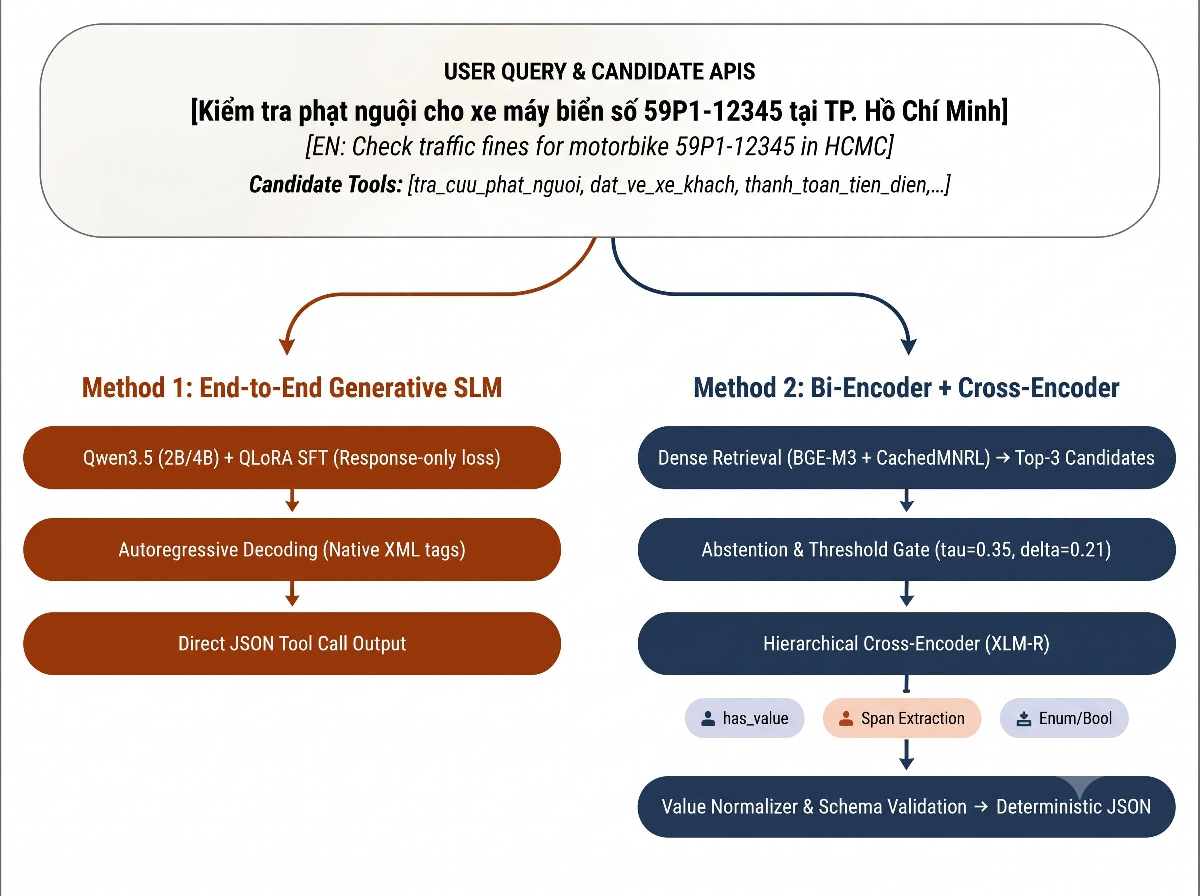
\includegraphics[width=0.88\textwidth]{figures/fig1_system_architecture}
    \caption{Sơ đồ kiến trúc đối chiếu giữa Phương pháp 1 và Phương pháp 2}
    \label{fig:hình_4_1}
\end{figure}

\textit{Hình 4.1: Sơ đồ kiến trúc đối chiếu giữa Phương pháp 1 (SLM End-to-End) và Phương pháp 2 (Bi-Encoder + Cross-Encoder).}

\section{Phương pháp 1: SLM End-to-End dựa trên Qwen3.5 (2B và 4B)}
Phương pháp 1 tiếp cận bài toán theo trường phái tạo sinh nguyên khối (End-to-End Generative Approach). Trong mô hình này, mạng nơ-ron tiếp nhận toàn bộ định nghĩa các công cụ khả dụng cùng câu truy vấn của người dùng trong cùng một cửa sổ ngữ cảnh duy nhất. Cơ chế tự chú ý (Self-Attention) cho phép mô hình liên kết trực tiếp các điều kiện ràng buộc trong mô tả API với các thực thể trong câu hỏi, từ đó tự hồi quy sinh ra cấu trúc lệnh gọi công cụ theo định dạng XML chuẩn của họ mô hình Qwen3.5:

\begin{verbatim}
<tool_call>
<function=tra_cuu_phat_nguoi>
<parameter=bien_so>30A-999.88</parameter>
<parameter=loai_phuong_tien>o_to</parameter>
</function>
</tool_call>
\end{verbatim}
Khi câu truy vấn chỉ mang tính giao tiếp thông thường hoặc không có công cụ nào trong hệ thống đáp ứng được yêu cầu, mô hình sẽ trực tiếp sản sinh câu trả lời bằng ngôn ngữ tự nhiên và từ chối tạo lập thẻ \texttt{<tool_call>}. Cơ chế này giúp hợp nhất năng lực đàm thoại tự nhiên và khả năng gọi hàm vào một mô hình thống nhất.

\textbf{Quy trình huấn luyện và thiết lập siêu tham số}:
Mô hình được tinh chỉnh trên hạ tầng GPU NVIDIA A100-40GB thông qua thư viện Unsloth và chuẩn kỹ thuật QLoRA 4-bit với các siêu tham số được mô tả chi tiết tại Bảng 4.1.


\begin{table}[htbp]
    \centering
    \caption{Thiết lập siêu tham số huấn luyện mô hình SLM Qwen3.5 (2B và 4B)}
    \label{tab:bảng_4_1}
    \begin{tabular}{lcc}
        \toprule
        \textbf{Siêu tham số (Hyperparameter)} & \textbf{Qwen3.5-2B} & \textbf{Qwen3.5-4B} \\
        \midrule
        \textbf{Kỹ thuật lượng tử hóa (Quantization)} & 4-bit NormalFloat (NF4) & 4-bit NormalFloat (NF4) \\
        \textbf{Hạng thích ứng LoRA ($r$)} & 16 & 16 \\
        \textbf{Hệ số tỷ lệ LoRA ($\alpha$)} & 16 & 16 \\
        \textbf{Target Modules} & Toàn bộ Q, K, V, O, Gate, Up, Down Proj & Toàn bộ Q, K, V, O, Gate, Up, Down Proj \\
        \textbf{Tốc độ học (Learning Rate)} & $5 \times 10^{-7}$ & $5 \times 10^{-7}$ \\
        \textbf{Bộ lập lịch tốc độ học (Scheduler)} & Cosine decay & Cosine decay \\
        \textbf{Batch Size cấu hình} & $64 \times 1$ (Per-device: 64, Accum: 1) & $32 \times 2$ (Per-device: 32, Accum: 2) \\
        \textbf{Batch Size hiệu dụng (Effective BS)} & \textbf{64} (Đồng nhất 100\%) & \textbf{64} (Đồng nhất 100\%) \\
        \textbf{Thuật toán tối ưu (Optimizer)} & AdamW 8-bit (\texttt{adamw_8bit}) & AdamW 8-bit (\texttt{adamw_8bit}) \\
        \textbf{Tỷ lệ khởi động ấm (Warmup Ratio)} & $0.05$ ($5\%$) & $0.05$ ($5\%$) \\
        \textbf{Hệ số tắt dần LoRA (Dropout)} & $0.0$ & $0.0$ \\
        \textbf{Độ dài ngữ cảnh tối đa (Max Length)} & $2{,}048$ tokens & $2{,}048$ tokens \\
        \textbf{Định dạng dữ liệu tính toán} & bfloat16 (BF16) & bfloat16 (BF16) \\
        \textbf{Kỹ thuật Gradient Checkpointing} & Kích hoạt (Unsloth Fast Gradient) & Kích hoạt (Unsloth Fast Gradient) \\
        \textbf{Tính toán hàm mất mát (Loss Masking)} & Chỉ tính trên phản hồi của Assistant & Chỉ tính trên phản hồi của Assistant \\
        \bottomrule
    \end{tabular}
\end{table}

Hệ thống siêu tham số trên được áp dụng đồng bộ và nhất quán xuyên suốt các chu trình huấn luyện (từ các cấu hình thực nghiệm đơn ngữ E1, E2 đến cấu hình song ngữ E3 và thích ứng miền chuyên biệt E4), bảo đảm tính kiểm soát biến số và khả năng đối sánh khách quan giữa các giai đoạn nghiên cứu.

\section{Phương pháp 2: Kiến trúc Phân tách Bi-Encoder + Cross-Encoder}

Phương pháp 2 chia bài toán thành hai giai đoạn: Bi-Encoder truy hồi công cụ theo ngữ nghĩa và Cross-Encoder trích xuất tham số theo lược đồ. Thiết kế mô-đun cho phép đánh giá riêng từng thành phần. Đầu ra được kiến tạo từ schema nên không ghi nhận lỗi cú pháp trong protocol hiện tại; độ trễ P50 tăng từ 55.13 ms tại $N=3$ lên 107.68 ms tại $N=1000$ trong stress test.

\section{1. Module Truy hồi Công cụ Ngữ nghĩa (Semantic Tool Retriever)}
Module đầu tiên chịu trách nhiệm thu hẹp không gian tìm kiếm từ kho hàng nghìn công cụ xuống một tập ứng viên rút gọn. Nhóm nghiên cứu sử dụng kiến trúc mạng hai tháp (Bi-Encoder) dựa trên nền tảng mô hình nhúng đa ngôn ngữ \texttt{BAAI/bge-m3}. Quá trình tối ưu hóa mô hình được triển khai thông qua quy trình huấn luyện hai vòng (two-round training): vòng thứ nhất huấn luyện mô hình cơ sở (teacher model) với hàm mất mát xếp hạng đa mẫu âm tính có bộ đệm (\texttt{CachedMNRL}); vòng thứ hai thực hiện khai thác các mẫu âm tính khó (hard negative mining) từ chính các dự đoán sai lệch của vòng 1 để tái huấn luyện mô hình cuối cùng.

Nhằm kiểm soát khả năng từ chối gọi công cụ đối với các câu hội thoại thông thường, hệ thống tích hợp cơ chế hiệu chuẩn ngưỡng kép (dual-threshold calibration) dựa trên điểm tương đồng ngữ nghĩa. Trong run Shared E4, ngưỡng tuyệt đối được hiệu chuẩn là $\tau = 0.35$ và ngưỡng biên tương đối là $\delta = 0.21$. Một công cụ mục tiêu chỉ được chấp thuận kích hoạt khi điểm tương đồng cao nhất thỏa mãn $s_{\max} \ge \tau$ và khoảng cách giữa điểm tương đồng Top-1 so với Top-2 đạt $s_{\text{top1}} - s_{\text{top2}} \ge \delta$. Các trường hợp không thỏa điều kiện được dự đoán là No-call.

\section{2. Module Trích xuất Tham số Phân cấp (Hierarchical Parameter Extractor)}
Sau khi công cụ mục tiêu được xác định, module thứ hai tiếp nhận chuỗi truy vấn của người dùng cùng với lược đồ thuộc tính (Tool Schema) của công cụ đó để trích xuất các giá trị tham số tương ứng. Module được xây dựng trên nền tảng mô hình biến đổi đa ngôn ngữ \texttt{xlm-roberta-base} với kiến trúc đầu ra phân cấp theo định hướng schema (Schema-driven routing).

Hệ thống sử dụng metadata của schema để định tuyến theo kiểu tham số. Đầu \texttt{has_value} dự đoán tham số có xuất hiện hay không; nếu có, \texttt{span_head}, \texttt{enum_head} hoặc \texttt{bool_head} xử lý theo kiểu dữ liệu tương ứng. Cơ chế giới hạn miền đầu ra cho enum và boolean, nhưng lỗi định tuyến hoặc dự đoán vẫn có thể khiến giá trị cuối cùng sai so với nhãn chuẩn.

\textbf{Quy chuẩn dữ liệu huấn luyện và hiệu chuẩn Method 2 (Shared E4)}:
Phương pháp 2 dùng cùng nguồn ngữ liệu hội thoại Shared E4 với SLM, gồm $65{,}600$ bản ghi gốc ($30{,}000$ EN, $30{,}000$ VI và $5{,}600$ CustomTools-VI Seen). Hai kiến trúc chuyển đổi bản ghi thành ví dụ huấn luyện khác nhau, nên việc dùng chung nguồn dữ liệu không bảo đảm mọi điều kiện huấn luyện và đo lường tương đương.

Trong khâu huấn luyện Bi-Encoder (\texttt{BAAI/bge-m3} tích hợp LoRA $r=16, \alpha=32$), hệ thống trích xuất chính xác $70{,}988$ cặp dương tính \texttt{(query, tool_description)} để lan truyền gradient tối ưu hóa hàm mất mát \texttt{CachedMNRL}. Toàn bộ 20 công cụ thuộc tập \texttt{unseen} bị loại trừ nghiêm ngặt khỏi dữ liệu huấn luyện dương tính, âm tính ngẫu nhiên cũng như quy trình khai thác mẫu âm khó nhằm duy trì tính độc lập hoàn toàn của miền zero-shot (\textit{Strict Zero-Shot Isolation}). Các mẫu không kích hoạt công cụ (no-call) không tham gia tính toán gradient thứ hạng mà được bảo lưu độc lập phục vụ cho việc hiệu chuẩn bộ tham số ngưỡng quyết định ($\tau = 0.35, \delta = 0.21$) trên tập kiểm định.

Đối với khâu huấn luyện Cross-Encoder (\texttt{xlm-roberta-base} với kiến trúc Hierarchical Heads), ngữ liệu được phân rã thành $135{,}617$ cặp \texttt{(query, param_schema)} gióng hàng trực tiếp, phục vụ huấn luyện liên hợp đầu nhị phân \texttt{has_value} và ba nhánh phân cấp chuyên biệt. Quy trình kiểm thử đối chuẩn sau đó được triển khai đồng bộ trên toàn bộ $7{,}712$ mẫu kiểm thử Core tiếng Việt (gồm $7{,}221$ mẫu có lệnh gọi và $491$ mẫu âm tính), $7{,}712$ mẫu Core tiếng Anh và hai tập kiểm thử \texttt{CustomTools-VI} Seen/Unseen với mỗi tập $800$ mẫu cân bằng 50\% âm tính.

Chi tiết toàn bộ cấu hình siêu tham số và tài nguyên tính toán của Phương pháp 2 được tổng hợp tại Bảng 4.2.


\begin{table}[htbp]
    \centering
    \caption{Thiết lập siêu tham số huấn luyện Phương pháp 2 (BGE-M3 và XLM-R)}
    \label{tab:bảng_4_2}
    \begin{tabular}{lll}
        \toprule
        \textbf{Thành phần kỹ thuật} & \textbf{Bộ truy hồi Bi-Encoder (BGE-M3)} & \textbf{Bộ trích xuất Cross-Encoder (XLM-R)} \\
        \midrule
        \textbf{Kiến trúc mô hình gốc} & \texttt{BAAI/bge-m3} (Dense Bi-Encoder) & \texttt{xlm-roberta-base} (Hierarchical Cross-Encoder) \\
        \textbf{Kỹ thuật thích ứng (PEFT)} & LoRA ($r=16, \alpha=32$, dropout $0.05$) & Huấn luyện liên hợp toàn diện (End-to-End Head Tuning) \\
        \textbf{Target Modules (LoRA)} & \texttt{query}, \texttt{key}, \texttt{value}, \texttt{dense} & — \\
        \textbf{Chiều dài chuỗi tối đa} & 192 tokens & 256 tokens (Question: 96, Context: 160) \\
        \textbf{Kích thước Batch (Batch size)} & 256 (Mini-batch: 32) & 32 (Gradient Accumulation Steps: 2 $\to$ 64) \\
        \textbf{Tốc độ học (Learning Rate)} & $2 \times 10^{-5}$ & Core: $3 \times 10^{-5}$, Custom: $1 \times 10^{-5}$, Heads: $1 \times 10^{-4}$ \\
        \textbf{Chiến lược huấn luyện} & 2 Rounds (Round 1 Teacher $\to$ Hard Negative Mining) & Curriculum Learning (2 Epochs Core $\to$ 2 Epochs Custom) \\
        \textbf{Hàm mất mát (Loss function)} & \texttt{CachedMultipleNegativesRankingLoss} & Binary Cross-Entropy (\texttt{has_value}, \texttt{bool}) + Cross-Entropy (\texttt{span}, \texttt{enum}) \\
        \textbf{Quy chuẩn quyết định (Policy)} & Gap selection: $\tau = 0.35, \delta = 0.21, k_{\max} = 3$ & Schema-driven routing + Regex Value Normalizer \\
        \textbf{Thời gian huấn luyện (Tesla T4)} & 6.15 giờ (Round 2 trên $70{,}988$ cặp dương tính) & 0.72 giờ ($4{,}240$ bước tối ưu hóa trên $135{,}617$ cặp) \\
        \textbf{Đỉnh chiếm dụng VRAM huấn luyện} & $10{,}888$ MB & $7{,}693$ MB \\
        \bottomrule
    \end{tabular}
\end{table}

\section{Cơ chế chuẩn hóa giá trị thực thể tiếng Việt (Vietnamese Value Normalizer)}

Đầu \texttt{span_head} của Cross-Encoder trích chuỗi xuất hiện trong truy vấn, còn API yêu cầu giá trị đúng kiểu và định dạng theo JSON Schema. Chẳng hạn, chuỗi \texttt{"hai triệu rưỡi"} không thể dùng trực tiếp cho tham số kiểu số. Vì vậy, Method 2 cần bước chuyển đổi giá trị trước khi tạo lời gọi.

Module Chuẩn hóa Giá trị tiếng Việt (Vietnamese Value Normalizer) sử dụng các quy tắc xác định qua bốn giai đoạn:

Giai đoạn 1 tách các biểu thức định lượng và ánh xạ từ lóng tiền tệ: “củ”, “chai” tương ứng $10^6$ đồng; “lít”, “xị”, “loét” tương ứng $10^5$ đồng; “cành”, “k” tương ứng $10^3$ đồng. Từ “rưỡi” biểu thị nửa đơn vị đứng trước, nên “hai củ rưỡi” được chuẩn hóa thành $2{,}500{,}000$ đồng.

Giai đoạn 2 phân tích số viết bằng chữ tiếng Việt theo thứ bậc tỷ, triệu, nghìn, trăm và hàng chục. Bộ phân tích cũng xử lý các biến thể như “lăm”, “nhăm”, “mươi” và “chục” để trả về giá trị số.

Giai đoạn 3 chuẩn hóa ngày tháng và mã định danh có cấu trúc. Các biểu thức thời gian được quy về ngày tuyệt đối theo thời điểm neo của hệ thống và định dạng ISO-8601 (\texttt{YYYY-MM-DD}). Với biển số và mã giao dịch, các quy tắc biểu thức chính quy xử lý khoảng trắng, dấu gạch ngang và chữ hoa; ví dụ, \texttt{"59 x1 999.88"} thành \texttt{"59X1-999.88"}.

Giai đoạn 4 ép giá trị theo kiểu khai báo tại \texttt{tools[].parameters.properties[key].type}, gồm \texttt{int}, \texttt{float}, \texttt{bool} hoặc chuỗi đã làm sạch. Đầu ra vẫn cần được xác thực theo JSON Schema trước khi thực thi; tỷ lệ lỗi cú pháp 0\% không có nghĩa là mọi tham số đều đúng nhãn chuẩn.

Hình 4.2 tóm tắt bốn giai đoạn xử lý.

\begin{verbatim}
graph LR
    classDef io fill:#e1f5fe,stroke:#0288d1,stroke-width:2px,color:#01579b;
    classDef step fill:#f3e5f5,stroke:#7b1fa2,stroke-width:2px,color:#4a148c;

    Raw["Chuỗi văn bản thô trích xuất từ span_head"]:::io
    S1["Bước 1: Phân đoạn từ vựng & Ánh xạ từ lóng<br/>('hai củ rưỡi' -> 2,500,000, 'năm xị' -> 500,000)"]:::step
    S2["Bước 2: Phân tích cú pháp số chữ tiếng Việt<br/>(Giải mã đệ quy hàng đơn vị, chục, trăm, triệu)"]:::step
    S3["Bước 3: Chuẩn hóa Regex có cấu trúc<br/>(Định dạng biển số xe, ngày tháng ISO-8601)"]:::step
    S4["Bước 4: Áp đặt kiểu dữ liệu theo Schema<br/>(Ép kiểu nguyên thủy integer, float, bool, string)"]:::step
    Clean["Giá trị tham số chuẩn hóa (JSON Compliant)"]:::io

    Raw --> S1
    S1 --> S2
    S2 --> S3
    S3 --> S4
    S4 --> Clean
\end{verbatim}

\textit{Hình 4.2: Quy trình bốn giai đoạn của module Chuẩn hóa Giá trị tiếng Việt (Vietnamese Value Normalizer).}


\chapter{THỰC NGHIỆM, ĐÁNH GIÁ VÀ BÀN LUẬN KẾT QUẢ}

\section{Thiết lập thực nghiệm và hạ tầng phần cứng}

Các mô hình SLM của Phương pháp 1 (\texttt{Qwen3.5-2B} và \texttt{Qwen3.5-4B}) được huấn luyện trên Google Colab Pro với một GPU NVIDIA A100-SXM4-40GB (bộ nhớ khả dụng 39.49 GB), RAM 83.5 GB, Ubuntu 22.04 LTS, CUDA 12.4 và PyTorch 2.5. Nhóm sử dụng Unsloth [16] và QLoRA 4-bit NF4 [6]. Hai thành phần Bi-Encoder (\texttt{BGE-M3}) và Cross-Encoder (\texttt{xlm-roberta-base}) của Phương pháp 2 được huấn luyện độc lập trên GPU NVIDIA Tesla T4 16GB thuộc Kaggle. Do phần cứng và quy trình khác nhau, các số đo vận hành của hai phương pháp cần được diễn giải theo từng protocol.

Khi đánh giá, Method 1 chia dữ liệu thành hai phần và suy luận độc lập trên 2× NVIDIA Tesla T4 của Kaggle. Cách chia này rút ngắn thời gian chạy toàn tập, nhưng không giảm độ trễ của một truy vấn. Method 2 được đo trên 1× T4, batch size 1, có cache embedding công cụ và đồng bộ CUDA quanh từng truy vấn; phép đo Core dùng ba lượt warm-up cho mỗi tập.

Bảng 5.2 báo cáo độ trễ mean trên Core VI. Trong stress test, số đo của SLM là thời gian batch chia theo số mẫu, còn Method 2 báo cáo P50/P95 theo từng truy vấn. Các bước có ngẫu nhiên dùng seed 42; nghiên cứu chưa lặp nhiều seed để ước lượng độ lệch chuẩn hoặc khoảng tin cậy.

Đường dẫn tới mã nguồn, dữ liệu và các checkpoint được tập hợp tại Phụ lục A để đối chiếu từng cấu hình thực nghiệm.

\section{Hệ thống độ đo đánh giá (Evaluation Metrics)}

Tham khảo BFCL [4] và nghiên cứu của Ersoy và cộng sự [1], khóa luận sử dụng năm độ đo định lượng cho độ chính xác nội dung, khả năng từ chối, tính hợp lệ định dạng và độ trễ. Định nghĩa cụ thể dưới đây áp dụng cho protocol của khóa luận, không đồng nhất với toàn bộ thước đo ở các công trình nguồn.

Độ chính xác lựa chọn công cụ (Tool Selection Accuracy - $\text{Tool Acc}$, \%) phản ánh khả năng định tuyến đúng công cụ mục tiêu từ yêu cầu của người dùng. Chỉ số này được tính toán trên tập các câu truy vấn dương tính, đòi hỏi danh sách công cụ dự đoán phải trùng khớp chính xác với nhãn tham chiếu cả về định danh lẫn thứ tự xuất hiện đối với các trường hợp đa lệnh gọi (multi-call):
$$\text{Tool Acc} = \frac{N_{\text{tool-exact, positive}}}{N_{\text{positive}}}$$

Độ chính xác khớp toàn bộ đầu ra (Argument Population Accuracy - $\text{ArgA}$, \%) là tiêu chuẩn đánh giá khắt khe nhất trong bài toán gọi công cụ, đại diện cho tỷ lệ các trường hợp mô hình thực hiện thành công trọn vẹn tác vụ. Một dự đoán chỉ được công nhận là chính xác khi mô hình chọn đúng công cụ đồng thời trích xuất hoàn hảo toàn bộ các cặp khóa–giá trị tham số mà không có bất kỳ sai lệch nào sau bước chuẩn hóa. Chỉ số báo cáo mặc định trên toàn bộ tập kiểm thử ($\text{ArgA}_{\text{all}}$) bao gồm cả các trường hợp nhận diện chính xác câu truy vấn không gọi hàm:
$$\text{ArgA}_{\text{all}} = \frac{N_{\text{exact, all}}}{N_{\text{all}}}$$
Bên cạnh đó, khi cần phân tích chuyên biệt trên nhóm câu hỏi đòi hỏi kích hoạt công cụ, độ chính xác tham số trên tập dương tính ($\text{ArgA}_{\text{positive}}$) được xác định bởi:
$$\text{ArgA}_{\text{positive}} = \frac{N_{\text{exact, positive}}}{N_{\text{positive}}}$$
Trong toàn bộ khóa luận, ký hiệu $\text{ArgA}$ được quy ước đại diện cho $\text{ArgA}_{\text{all}}$ trừ khi có diễn giải riêng.

Độ thu hồi từ chối gọi hàm (Non-Function-Calling Recall - $\text{Non-FC Recall}$, \%) đo lường năng lực nhận diện các câu thoại giao tiếp thông thường không chứa ý định kích hoạt API. Đây là thước đo mang tính quyết định nhằm phát hiện và kiểm soát hiện tượng thiên kiến kích hoạt quá mức (over-triggering pathology) trong các hệ thống tác tử thực tế:
$$\text{Non-FC Recall} = \frac{N_{\text{true negative}}}{N_{\text{negative}}}$$

Tỷ lệ lỗi cú pháp (Syntax Error Rate, \%) xác định tỷ lệ đầu ra không thể được bộ phân tích cú pháp xử lý theo định dạng đánh giá. Với Method 2, đầu ra được kiến tạo từ schema nên protocol hiện tại không ghi nhận lỗi cú pháp; kết quả 0\% chỉ phản ánh tính hợp lệ về định dạng, không chứng tỏ chọn đúng công cụ hay điền đúng tham số và không thay thế chỉ số ArgA.

Cuối cùng, độ trễ suy luận (Wall-clock Latency, ms) lượng hóa thời gian từ khi tiếp nhận truy vấn đến khi tạo xong đầu ra. Khóa luận ghi rõ mean hoặc phân vị P50/P95, tập mẫu, phần cứng và phạm vi tính thời gian cho từng phép đo; những số liệu từ các protocol khác nhau chỉ dùng để mô tả, không tạo thành phép đo tốc độ đối chứng đồng nhất.

\section{Kết quả tổng thể và giải đáp 5 câu hỏi nghiên cứu}

Kết quả trên \texttt{CustomTools-VI} gồm 1,600 mẫu seen/unseen được trình bày ở Bảng 5.1a và 5.1b. Bảng 5.2 báo cáo kết quả trên 7,712 mẫu kiểm thử của mỗi ngôn ngữ trong \texttt{Canonical Core Benchmark}. Các bảng này là cơ sở phân tích năm câu hỏi nghiên cứu RQ1–RQ5.


\begin{table}[htbp]
    \centering
    \caption{a: Kết quả thực nghiệm trên tập kiểm thử CustomTools-VI Seen}
    \label{tab:bảng_5_1}
    \resizebox{\textwidth}{!}{%
    \begin{tabular}{llcccc}
        \toprule
        \textbf{Mô hình} & \textbf{Cấu hình huấn luyện} & \textbf{Tool Acc (\%)} & \textbf{ArgA (\%)} & \textbf{Non-FC Recall (\%)} & \textbf{Syntax Error (\%)} \\
        \midrule
        \textbf{Nhóm SLM cục bộ} &  &  &  &  &  \\
        \textbf{Qwen3.5-2B} & E0 (Zero-shot) & 39.25\% & 56.75\% & 97.75\% & 11.00\% \\
        \textbf{Qwen3.5-2B} & E1 (Đơn ngữ EN 60k) & 91.50\% & 63.12\% & 75.25\% & 4.50\% \\
        \textbf{Qwen3.5-2B} & E2 (Đơn ngữ VI 60k) & 91.00\% & 51.50\% & 67.50\% & 7.18\% \\
        \textbf{Qwen3.5-2B} & E3 (Song ngữ 60k) & 92.25\% & 19.38\% & 3.00\% & 4.31\% \\
        \textbf{Qwen3.5-2B} & E4 (Song ngữ + Miền VI) & 93.25\% & 87.00\% & \textbf{100.00\%} & 2.44\% \\
        \textbf{Qwen3.5-4B} & E3 (Song ngữ 60k) & 92.00\% & 62.00\% & 71.25\% & 12.00\% \\
        \textbf{Qwen3.5-4B} & \textbf{E4 (Song ngữ + Miền VI)} & \textbf{94.66\%} & \textbf{87.92\%} & \textbf{100.00\%} & 2.90\% \\
        \textbf{Nhóm Method 2 phân tách} &  &  &  &  &  \\
        \textbf{Method 2} & Bi-Encoder + Cross-Encoder & 92.25\% & 85.38\% & 92.75\% & \textbf{0.00\%} \\
        \textbf{Nhóm Frontier API đám mây} &  &  &  &  &  \\
        \textbf{GPT-5.6 Luna} & OpenAI API (không truyền tham số nhiệt độ) & 93.25\% & 78.25\% & 100.00\% & 0.00\% \\
        \textbf{Gemini 3.8 Flash} & Google API (không truyền tham số nhiệt độ) & \textbf{100.00\%} & \textbf{93.62\%} & 100.00\% & 0.06\% \\
        \bottomrule
    \end{tabular}
    }%
\end{table}

\textit{Ghi chú Bảng 5.1a: Các chỉ số được tính trên tập \texttt{test_seen} gồm 800 mẫu, với 400 mẫu dương tính và 400 mẫu âm tính. Tool Acc tính trên mẫu dương tính; ArgA tính trên toàn bộ mẫu; Non-FC Recall tính trên mẫu âm tính. Với Method 2, 0\% lỗi cú pháp là hệ quả của việc kiến tạo đầu ra theo schema, không đồng nghĩa với ArgA đạt 100\%. Mã benchmark API không truyền \texttt{temperature}; không thể quy kết kết quả cho cấu hình $T=0$.}


\begin{table}[htbp]
    \centering
    \caption{b: Kết quả thực nghiệm trên tập kiểm thử CustomTools-VI Unseen}
    \label{tab:bảng_5_1}
    \resizebox{\textwidth}{!}{%
    \begin{tabular}{llcccc}
        \toprule
        \textbf{Mô hình} & \textbf{Cấu hình huấn luyện} & \textbf{Tool Acc (\%)} & \textbf{ArgA (\%)} & \textbf{Non-FC Recall (\%)} & \textbf{Syntax Error (\%)} \\
        \midrule
        \textbf{Nhóm SLM cục bộ} &  &  &  &  &  \\
        \textbf{Qwen3.5-2B} & E0 (Zero-shot) & 40.75\% & 62.50\% & 97.25\% & 11.00\% \\
        \textbf{Qwen3.5-2B} & E1 (Đơn ngữ EN 60k) & 96.50\% & 70.50\% & 74.50\% & 4.50\% \\
        \textbf{Qwen3.5-2B} & E2 (Đơn ngữ VI 60k) & 96.25\% & 59.62\% & 67.75\% & 7.18\% \\
        \textbf{Qwen3.5-2B} & E3 (Song ngữ 60k) & 96.00\% & 27.88\% & 2.00\% & 4.31\% \\
        \textbf{Qwen3.5-2B} & E4 (Song ngữ + Miền VI) & 97.00\% & 86.38\% & \textbf{100.00\%} & 2.44\% \\
        \textbf{Qwen3.5-4B} & E3 (Song ngữ 60k) & 97.50\% & 69.75\% & 74.50\% & 12.00\% \\
        \textbf{Qwen3.5-4B} & \textbf{E4 (Song ngữ + Miền VI)} & 96.75\% & \textbf{86.75\%} & \textbf{100.00\%} & 2.90\% \\
        \textbf{Nhóm Method 2 phân tách} &  &  &  &  &  \\
        \textbf{Method 2} & Bi-Encoder + Cross-Encoder & 79.50\% & 60.25\% & 93.75\% & \textbf{0.00\%} \\
        \textbf{Nhóm Frontier API đám mây} &  &  &  &  &  \\
        \textbf{GPT-5.6 Luna} & OpenAI API (không truyền tham số nhiệt độ) & 97.25\% & 79.50\% & 100.00\% & 0.00\% \\
        \textbf{Gemini 3.8 Flash} & Google API (không truyền tham số nhiệt độ) & \textbf{100.00\%} & \textbf{92.12\%} & 99.75\% & 0.06\% \\
        \bottomrule
    \end{tabular}
    }%
\end{table}

\textit{Ghi chú Bảng 5.1b: Các chỉ số được tính trên tập \texttt{test_unseen} gồm 800 mẫu, với 400 mẫu dương tính và 400 mẫu âm tính. Tool Acc tính trên mẫu dương tính; ArgA tính trên toàn bộ mẫu; Non-FC Recall tính trên mẫu âm tính. Với Method 2, 0\% lỗi cú pháp là hệ quả của việc kiến tạo đầu ra theo schema, không đồng nghĩa với ArgA đạt 100\%. Mã benchmark API không truyền \texttt{temperature}; không thể quy kết kết quả cho cấu hình $T=0$.}

\begin{figure}[htbp]
    \centering
    
\includegraphics[width=0.88\textwidth]{figures/fig2_performance_comparison}
    \caption{So sánh hiệu năng các phương pháp trên benchmark CustomTools-VI}
    \label{fig:hình_5_1}
\end{figure}

\textit{Hình 5.1: So sánh hiệu năng các phương pháp trên benchmark CustomTools-VI (Seen vs. Unseen).}



\begin{table}[htbp]
    \centering
    \caption{Kết quả thực nghiệm trên Canonical Core Benchmark (7,712 mẫu)}
    \label{tab:bảng_5_2}
    \resizebox{\textwidth}{!}{%
    \begin{tabular}{llccccccc}
        \toprule
        \textbf{Mô hình} & \textbf{Cấu hình huấn luyện} & \textbf{VI Test: Tool Acc (\%)} & \textbf{VI Test: ArgA (\%)} & \textbf{VI Test: Non-FC (\%)} & \textbf{EN Test: Tool Acc (\%)} & \textbf{EN Test: ArgA (\%)} & \textbf{EN Test: Non-FC (\%)} & \textbf{Độ trễ VI mean (ms)} \\
        \midrule
        \textbf{Qwen3.5-2B} & E0 (Zero-Shot) & 56.34\% & 40.48\% & 96.33\% & 85.18\% & 60.63\% & 94.50\% & 707 ms \\
        \textbf{Qwen3.5-2B} & E1 (Đơn ngữ EN 60k) & 93.67\% & 65.57\% & 94.30\% & 94.07\% & \textbf{73.66\%} & 94.30\% & 878 ms \\
        \textbf{Qwen3.5-2B} & E2 (Đơn ngữ VI 60k) & 90.25\% & 64.90\% & 94.30\% & 93.45\% & 71.36\% & 93.08\% & 872 ms \\
        \textbf{Qwen3.5-2B} & E3 (Song ngữ 60k) & 94.00\% & 69.76\% & 94.30\% & 94.27\% & 73.22\% & 94.30\% & 864 ms \\
        \textbf{Qwen3.5-2B} & E4 (Song ngữ + Miền VI) & 93.92\% & 69.75\% & 94.30\% & 94.17\% & 73.15\% & 94.30\% & 970 ms \\
        \textbf{Qwen3.5-4B} & E3 (Song ngữ 60k) & \textbf{98.73\%} & \textbf{72.86\%} & 94.30\% & \textbf{96.63\%} & \textbf{74.71\%} & 94.30\% & 2,432 ms \\
        \textbf{Qwen3.5-4B} & E4 (Song ngữ + Miền VI) & 86.22\% & 64.94\% & 94.30\% & 85.03\% & 66.66\% & 94.30\% & 2,485 ms \\
        \textbf{Method 2} & Shared E4 (Bi+Cross) & 59.20\% & 30.26\% & 94.09\% & 62.60\% & 35.52\% & 94.30\% & \textbf{61.50 ms} \\
        \bottomrule
    \end{tabular}
    }%
\end{table}

\textit{Ghi chú: Cột độ trễ báo cáo mean trên Core VI. SLM chia dữ liệu trên 2× T4 và suy luận độc lập từng phần, không tăng tốc một truy vấn; Method 2 đo trên 1× T4, batch 1, có cache embedding công cụ và đồng bộ CUDA quanh từng truy vấn (P50 = 59.55 ms). Method 2 được đánh giá trên đủ 7,712 mẫu của mỗi ngôn ngữ. Do phạm vi xử lý và protocol đo khác nhau, không tính tỷ lệ tăng tốc trực tiếp từ cột này.}


\section{1. RQ1: Năng lực chuyển giao tri thức ngôn ngữ chéo (Cross-Lingual Transfer)}

Trên Core VI (Bảng 5.2), E1 chỉ huấn luyện bằng tiếng Anh đạt \textbf{65.57\%} ArgA, cao hơn E2 chỉ huấn luyện bằng tiếng Việt (\textbf{64.90\%}). Trên CustomTools-VI Unseen, hai cấu hình lần lượt đạt \textbf{70.50\%} và \textbf{59.62\%}. Những kết quả này cho thấy E1 vẫn xử lý được truy vấn tiếng Việt trong hai tập đánh giá.

Hiện tượng thực nghiệm này phù hợp với giả thuyết rằng Qwen3.5 chuyển giao được một phần năng lực phân tích schema từ tiếng Anh sang tiếng Việt. Tuy nhiên, thiết kế hiện tại chưa tách riêng tác động của tiền huấn luyện đa ngôn ngữ và dữ liệu tinh chỉnh. Ở chiều đánh giá ngược trên Core EN, E2 đạt 71.36\% so với 73.66\% của E1; E3 đạt ArgA 69.76\% trên Core VI ở mô hình 2B và 72.86\% ở mô hình 4B. Các kết quả cho thấy sự khác biệt giữa cấu hình dữ liệu trong những lần chạy này, chưa chứng minh E3 giải quyết hoàn toàn mất cân bằng ngôn ngữ.

\section{2. RQ2: Hiện tượng kích hoạt công cụ quá mức và vai trò của dữ liệu âm tính}

Trên CustomTools-VI, E3 được huấn luyện bằng 60,000 mẫu song ngữ nhưng không có dữ liệu âm tính đặc thù miền. Non-FC Recall chỉ đạt \textbf{2.00\%–3.00\%}, nghĩa là mô hình gọi công cụ nhầm ở hơn 97\% truy vấn âm tính trong hai tập kiểm thử. Đây là biểu hiện của thiên kiến kích hoạt công cụ quá mức (over-triggering) trong điều kiện đánh giá này.

Trên CustomTools-VI, ArgA-all của SLM 2B E3 đạt \textbf{19.38\%} ở seen và \textbf{27.88\%} ở unseen. Sau khi bổ sung 5,600 mẫu bản địa ở E4, trong đó có mẫu âm tính, Non-FC Recall đạt \textbf{100.00\%} trên cả hai tập kiểm thử; ArgA-all tăng lên \textbf{87.00\%} và \textbf{86.38\%}. Chênh lệch phù hợp với giả thuyết dữ liệu bản địa hỗ trợ nhận diện truy vấn không gọi hàm, nhưng E3 và E4 khác nhau ở nhiều khía cạnh dữ liệu nên chưa xác định riêng tác động của mẫu âm tính.

\section{3. RQ3: Khả năng tổng quát hóa Zero-Shot trên công cụ chưa từng gặp}

Trên \texttt{test_unseen}, SLM E4 và Method 2 có mức suy giảm ArgA khác nhau so với \texttt{test_seen}.

SLM E4 đạt ArgA \textbf{86.38\%} ở bản 2B và \textbf{86.75\%} ở bản 4B trên tập unseen, chênh lần lượt $-0.62$ và $-1.17$ điểm phần trăm so với tập seen. Kết quả phù hợp với khả năng sử dụng mô tả công cụ và schema trong prompt để xử lý công cụ mới; phép đánh giá hiện tại chưa tách riêng tác động của từng thành phần này.

Method 2 đạt ArgA \textbf{85.38\%} trên \texttt{test_seen} và \textbf{60.25\%} trên \texttt{test_unseen}; ArgA của riêng truy vấn dương tính unseen là 26.75\%. Tool Acc giảm từ 92.25\% xuống 79.50\%. Các số liệu cho thấy cả việc chọn công cụ lẫn hoàn thiện lời gọi đều khó hơn trên tập unseen. Đối chứng Oracle ở Chương 6 giúp phân tích thêm vai trò của từng giai đoạn, nhưng chưa xác định nguyên nhân duy nhất của mức suy giảm.

\section{4. RQ4: Đánh đổi Pareto giữa độ chính xác, độ trễ và chi phí tính toán}

Nhằm cung cấp cơ sở khoa học phục vụ việc lựa chọn kiến trúc trong các kịch bản triển khai thực tế, Bảng 5.3 tổng hợp đường biên đánh đổi đa chiều giữa các phương pháp đại diện trên toàn bộ các trục tiêu chí kỹ thuật cốt lõi.


\begin{table}[htbp]
    \centering
    \caption{Đối chiếu chỉ số và điều kiện vận hành của bốn phương pháp}
    \label{tab:bảng_5_3}
    \resizebox{\textwidth}{!}{%
    \begin{tabular}{lccccl}
        \toprule
        \textbf{Trục đánh giá kỹ thuật} & \textbf{Method 1: SLM Qwen3.5-2B (E4)} & \textbf{Method 1: SLM Qwen3.5-4B (E4)} & \textbf{Method 2: Bi+Cross (BGE-M3 + XLM-R)} & \textbf{Frontier Closed: GPT-5.6 Luna} & \textbf{Khuyến nghị lựa chọn kỹ thuật} \\
        \midrule
        \textbf{Kiến trúc mô hình} & Tự hồi quy (Decoder-only) & Tự hồi quy (Decoder-only) & Phân tách phân biệt (Encoders) & Mô hình đám mây (Cloud API) & Tùy biến theo năng lực hạ tầng \\
        \textbf{Quy mô tham số} & 2.22 tỷ (QLoRA 10.9M) & 4.56 tỷ (QLoRA 21.2M) & 567M (Bi) + 278M (Cross) & Không công bố trong log đánh giá & Phụ thuộc kiến trúc và triển khai \\
        \textbf{Custom Seen ArgA} & 87.00\% & \textbf{87.92\%} & 85.38\% & 78.25\% & SLM E4 cao hơn Luna trên tập này \\
        \textbf{Custom Unseen ArgA} & 86.38\% & \textbf{86.75\%} & 60.25\% & 79.50\% & SLM E4 cao hơn trên tập này \\
        \textbf{Lỗi cú pháp CustomTools-VI} & 2.44\% & 2.90\% & \textbf{0.00\% (đầu ra kiến tạo từ schema)} & 0.00\% & Chỉ phản ánh định dạng; xem ArgA để đánh giá nội dung \\
        \textbf{Độ trễ Core VI mean (ms)\}* & 970 ms & 2,485 ms & \textbf{61.50 ms} & Không đo trên Core VI & Chỉ đối chiếu mô tả do protocol khác nhau \\
        \textbf{Mức tiêu thụ VRAM (đo đạc)\}* & ~4.8–5.5 GB VRAM & ~9.5 GB VRAM & \textbf{3,283 MiB allocated; 3,772 MiB reserved} & Không tiêu tốn VRAM cục bộ & Số liệu phụ thuộc protocol và công cụ đo \\
        \textbf{Khả năng mở rộng danh mục} & Giới hạn bởi cửa sổ ngữ cảnh & Giới hạn bởi cửa sổ ngữ cảnh & Đã kiểm thử với $N \le 1000$ & Chưa kiểm thử stress test & Cần đánh giá theo quy mô danh mục thực tế \\
        \textbf{Phạm vi quan sát} & Core VI và CustomTools-VI & Core VI và CustomTools-VI & Core VI, CustomTools-VI và stress test & CustomTools-VI & Chọn theo miền dữ liệu và điều kiện triển khai \\
        \bottomrule
    \end{tabular}
    }%
\end{table}

\textit{Ghi chú: SLM dùng hai T4 để chia dữ liệu và suy luận độc lập; một truy vấn chạy trên một GPU. Method 2 dùng một T4, batch 1 và cache embedding. Các số trong hàng độ trễ là mean Core VI của cấu hình E4, không phải P50; P50 từng truy vấn của Method 2 trong stress test nằm ở Bảng 5.4b. Hàng VRAM kết hợp số đo từ các run và cách ghi nhận khác nhau; riêng Method 2 là bộ nhớ PyTorch allocated/reserved tại $N=1000$. Protocol đo và phạm vi xử lý khác nhau nên các hàng này không chứng minh tỷ lệ tăng tốc hay mức tiết kiệm VRAM trực tiếp. API chỉ được kiểm thử trên CustomTools-VI.}

Các kết quả gợi ý hai lựa chọn kiến trúc theo yêu cầu triển khai. Trên CustomTools-VI unseen, SLM E4 đạt ArgA cao hơn Method 2, phù hợp với bài toán thường xuyên tiếp nhận schema mới. Trong protocol stress test với danh mục xác định trước, Method 2 ghi nhận P50 dưới 100 ms ở $N \le 500$, tiếp tục xử lý được $N=1000$ và không có lỗi cú pháp theo định nghĩa đầu ra kiến tạo từ schema. Khả năng áp dụng cho thiết bị biên và mục tiêu độ trễ sản xuất vẫn cần đo trên phần cứng, tải và quy trình phục vụ tương ứng.

\section{5. RQ5: Kiểm thử áp lực quy mô lớn và giới hạn vật lý của mô hình tạo sinh}

Để kiểm chứng tính bền bỉ của hai trường phái kiến trúc khi quy mô danh mục công cụ mở rộng từ dải nhỏ ($N = 3$) đến quy mô thực tế của các nền tảng doanh nghiệp ($N = 1000$ công cụ), nghiên cứu tiến hành bài kiểm thử áp lực (\textbf{Stress Test}) đối đầu trực diện giữa đại diện tiêu biểu của Method 1 (\texttt{Qwen3.5-2B} E4) và Method 2 trên cùng 200 truy vấn Custom Seen (1,200 mẫu thử nghiệm lồng nhau). Độ chính xác được báo cáo ở Bảng 5.4a, độ trễ và bộ nhớ ở Bảng 5.4b; Hình 5.2 trực quan hóa xu hướng theo $N$.


\begin{table}[htbp]
    \centering
    \caption{a: Độ chính xác trong Stress Test theo quy mô danh mục công cụ ($N = 3 \to 1000$)}
    \label{tab:bảng_5_4}
    \begin{tabular}{crrrr}
        \toprule
        \textbf{Số công cụ ($N$)} & \textbf{SLM Tool Acc (\%)} & \textbf{M2 Tool Acc (\%)} & \textbf{SLM ArgA (\%)} & \textbf{M2 ArgA (\%)} \\
        \midrule
        \textbf{3} & \textbf{94.0\%} & 89.0\% & 85.5\% & \textbf{87.5\%} \\
        \textbf{10} & \textbf{93.0\%} & 89.0\% & 84.5\% & \textbf{87.5\%} \\
        \textbf{50} & \textbf{93.0\%} & 89.0\% & 85.5\% & \textbf{87.5\%} \\
        \textbf{100} & \textbf{92.0\%} & 89.0\% & 83.0\% & \textbf{87.0\%} \\
        \textbf{500} & \textit{OOM} & \textbf{87.0\%} & \textit{OOM} & \textbf{85.0\%} \\
        \textbf{1000} & \textit{OOM} & \textbf{87.0\%} & \textit{OOM} & \textbf{84.0\%} \\
        \bottomrule
    \end{tabular}
\end{table}


\begin{table}[htbp]
    \centering
    \caption{b: Độ trễ và bộ nhớ trong Stress Test theo quy mô danh mục công cụ}
    \label{tab:bảng_5_4}
    \begin{tabular}{crrr}
        \toprule
        \textbf{Số công cụ ($N$)} & \textbf{Độ trễ SLM (ms)*} & \textbf{M2 P50 (ms)} & \textbf{M2 P95 (ms)} \\
        \midrule
        \textbf{3} & 1,258.94 & \textbf{55.13} & 84.92 \\
        \textbf{10} & 1,604.68 & \textbf{55.05} & 84.74 \\
        \textbf{50} & 4,703.39 & \textbf{56.07} & 86.46 \\
        \textbf{100} & 9,318.21 & \textbf{61.01} & 85.09 \\
        \textbf{500} & \textit{OOM} & \textbf{92.27} & 128.82 \\
        \textbf{1000} & \textit{OOM} & \textbf{107.68} & 148.21 \\
        \bottomrule
    \end{tabular}
\end{table}

\textit{Ghi chú Bảng 5.4b: Độ trễ SLM là thời gian sinh của batch chia cho số mẫu trong batch, với batch size thay đổi theo $N$; đây không phải P50 wall-clock từng truy vấn. Method 2 đo từng truy vấn ở batch 1, có đồng bộ CUDA và cache embedding. Hai phép đo khác giao thức, nên không quy đổi thành hệ số tăng tốc. PyTorch allocated VRAM của Method 2 tại $N=3, 10, 50, 100, 500, 1000$ lần lượt là 3,277; 3,282; 3,278; 3,283; 3,283; 3,283 MiB.}

\begin{figure}[htbp]
    \centering
    
\includegraphics[width=0.88\textwidth]{figures/fig3_stress_test_curves}
    \caption{Kết quả Stress Test đối đầu trực diện khi mở rộng quy mô công cụ ($N = 3 \to 1000$)}
    \label{fig:hình_5_2}
\end{figure}

\textit{Hình 5.2: Kết quả Stress Test đối đầu trực diện ($N = 3 \to 1000$): (a) Độ chính xác và ranh giới CUDA OOM của SLM tại $N \ge 500$; (b) Độ trễ suy luận trên thang log (P50 đơn truy vấn ở Method 2 và thời gian batch chia đều ở SLM).}

Thực nghiệm kiểm thử áp lực đã làm sáng tỏ những khác biệt mang tính bản chất trong cơ chế vận hành của hai mô thức thiết kế:

Trong stress test giữ nguyên tập truy vấn mỏ neo, ArgA của Method 2 giảm từ 87.50\% ở $N=3$ xuống 84.00\% ở $N=1000$, tức 3.50 điểm phần trăm. Ở $N \le 100$, ArgA của Method 2 cao hơn SLM từ 2.0 đến 4.0 điểm phần trăm; tại $N=1000$, Non-FC Recall của Method 2 là 95.00\%. Quan sát cho thấy cơ chế lọc ngưỡng ($\tau=0.35$, $\delta=0.21$) vẫn hoạt động trong protocol này, nhưng chưa tách riêng đóng góp của nó khỏi các thành phần khác.

Trong protocol stress test, P50 từng truy vấn của Method 2 nằm trong khoảng 55.05–61.01 ms ở $N \le 100$ và đạt 107.68 ms tại $N=1000$. Việc phải đối chiếu với nhiều vector công cụ hơn có thể góp phần làm tăng thời gian xử lý. Số đo SLM từ thời gian batch chia theo mẫu tăng từ 1,258.94 ms ($N=3$) lên 9,318.21 ms ($N=100$), phù hợp với việc prompt chứa thêm schema; hai chuỗi số liệu không cùng định nghĩa nên không dùng để tính hệ số tăng tốc.

Trong cấu hình stress test trên GPU 16GB, SLM gặp CUDA Out of Memory ở $N \ge 500$. Quan sát này phù hợp với giả thuyết rằng prompt dài làm tăng nhu cầu bộ nhớ ở các lớp attention toàn phần, song chưa đủ để tách riêng tác động của attention, KV cache, precision, batch và cách hiện thực kernel. Cấu hình Qwen3.5 được dùng còn xen kẽ các lớp linear attention và full attention [17], nên không thể dùng riêng độ phức tạp $\mathcal{O}(L^2)$ của full attention để giải thích toàn bộ hiện tượng. Method 2 tiếp tục chạy ở $N=1000$ và ghi nhận PyTorch allocated VRAM khoảng 3.21 GiB (3,283 MiB) trong protocol này.

\section{Nghiên cứu mở rộng quy mô mô hình: Qwen3.5-2B vs. Qwen3.5-4B}

Để làm sáng tỏ ảnh hưởng của dung lượng tham số đối với năng lực tiếp nhận schema phức tạp và tính ổn định cú pháp, quá trình huấn luyện được mở rộng lên mô hình \texttt{Qwen3.5-4B} (4.56 tỷ tham số). Kết quả đối chuẩn chi tiết được trình bày tại Bảng 5.5, Bảng 5.6 và minh họa tại Hình 5.3.


\begin{table}[htbp]
    \centering
    \caption{Nghiên cứu mở rộng quy mô tham số mô hình (Qwen3.5-2B vs. 4B)}
    \label{tab:bảng_5_5}
    \resizebox{\textwidth}{!}{%
    \begin{tabular}{llcccccc}
        \toprule
        \textbf{Cấu hình} & \textbf{Backbone} & \textbf{Core VI ArgA (\%)} & \textbf{Custom Seen ArgA (\%)} & \textbf{Custom Unseen ArgA (\%)} & \textbf{ArgA Gap} & \textbf{Cú pháp lỗi Core VI (\%)} & \textbf{Độ trễ Core VI mean (ms)} \\
        \midrule
        \textbf{E3 (Song ngữ)} & Qwen3.5-2B & 69.76\% & 19.38\% & 27.88\% & +8.50\% & 4.31\% & 864 ms \\
        \textbf{E3 (Song ngữ)} & \textbf{Qwen3.5-4B} & \textbf{72.86\%} & \textbf{62.00\%} & \textbf{69.75\%} & +7.75\% & \textbf{0.32\%} & 2,432 ms \\
        \textbf{E4 (Đặc thù miền)} & Qwen3.5-2B & 69.75\% & 87.00\% & 86.38\% & -0.62\% & 4.67\% & 970 ms \\
        \textbf{E4 (Đặc thù miền)} & \textbf{Qwen3.5-4B} & 64.94\% & \textbf{87.92\%} & \textbf{86.75\%} & \textbf{-1.17\%} & 9.75\% & 2,485 ms \\
        \bottomrule
    \end{tabular}
    }%
\end{table}


\begin{table}[htbp]
    \centering
    \caption{Hiệu năng đối đầu của mô hình Qwen3.5-4B (E3 vs. E4) trên Core Benchmark}
    \label{tab:bảng_5_6}
    \resizebox{\textwidth}{!}{%
    \begin{tabular}{llcccccc}
        \toprule
        \textbf{Cấu hình} & \textbf{Tập kiểm thử} & \textbf{Số mẫu (Samples)} & \textbf{Tool Selection Acc (\%)} & \textbf{ArgA / Exact Match (\%)} & \textbf{Non-FC Recall (\%)} & \textbf{Tỷ lệ lỗi cú pháp (\%)} & \textbf{Độ trễ trung bình (ms)} \\
        \midrule
        \textbf{E3 (Song ngữ)} & Core VI Test & 7,712 (7,221 pos / 491 neg) & \textbf{98.73\%} & \textbf{72.86\%} & 94.30\% & \textbf{0.32\%} & 2,431.83 ms \\
        \textbf{E3 (Song ngữ)} & Core EN Test & 7,712 (7,221 pos / 491 neg) & \textbf{96.63\%} & \textbf{74.71\%} & 94.30\% & \textbf{1.97\%} & 3,289.59 ms \\
        \textbf{E4 (Đặc thù miền)} & Core VI Test & 7,712 (7,221 pos / 491 neg) & 86.22\% & 64.94\% & 94.30\% & 9.75\% & 2,485.12 ms \\
        \textbf{E4 (Đặc thù miền)} & Core EN Test & 7,712 (7,221 pos / 491 neg) & 85.03\% & 66.66\% & 94.30\% & 11.36\% & 3,310.25 ms \\
        \bottomrule
    \end{tabular}
    }%
\end{table}

\begin{figure}[htbp]
    \centering
    
\includegraphics[width=0.88\textwidth]{figures/fig4_model_scaling}
    \caption{Nghiên cứu mở rộng quy mô tham số mô hình SLM (2B vs. 4B)}
    \label{fig:hình_5_3}
\end{figure}

\textit{Hình 5.3: So sánh mô hình 2B và 4B: (a) Độ chính xác chọn công cụ và trích xuất tham số trên Core Benchmark; (b) Tỷ lệ lỗi cú pháp JSON.}

Mục này so sánh kết quả của hai checkpoint Qwen3.5 có quy mô 2.22 tỷ và 4.56 tỷ tham số trong các cấu hình đã thử nghiệm.

Ở cấu hình song ngữ E3 trên Core VI, tỷ lệ vi phạm cú pháp giảm từ 4.31\% ở mô hình 2B xuống \textbf{0.32\%} ở mô hình 4B, tương đương mức giảm hơn 13 lần trong phép đo này. Chênh lệch phù hợp với giả thuyết mô hình lớn hơn tuân thủ định dạng tốt hơn, nhưng chưa chứng minh riêng quy mô tham số là nguyên nhân vì hai checkpoint có thể khác nhau ở nhiều yếu tố.

Trên Core VI, Qwen3.5-4B E3 đạt Tool Acc \textbf{98.73\%} và ArgA \textbf{72.86\%}, cao hơn bản 2B E3 lần lượt 4.73 và 3.10 điểm phần trăm. Phép so sánh này ghi nhận lợi thế của checkpoint 4B trong cấu hình E3, nhưng chưa tách riêng ảnh hưởng của quy mô tham số khỏi các khác biệt huấn luyện khác.

Trên CustomTools-VI, ArgA của 2B E3 là 19.38\% ở seen và 27.88\% ở unseen; 4B E3 lần lượt đạt 62.00\% và 69.75\%. Khoảng cách này cho thấy hai checkpoint phản ứng khác nhau với dữ liệu miền mới, song chưa đủ để quy toàn bộ khác biệt cho kích thước mô hình.

Sau khi bổ sung 5,600 mẫu nghiệp vụ Việt Nam ở E4, Qwen3.5-4B đạt ArgA \textbf{87.92\%} trên seen và \textbf{86.75\%} trên unseen của CustomTools-VI. Trên Core VI, ArgA của E4 còn 64.94\% và tỷ lệ lỗi cú pháp là 9.75\%. Vì vậy, lựa chọn giữa E3 và E4 cần dựa trên miền dữ liệu mục tiêu; kết quả hiện có không bảo đảm checkpoint nào tốt hơn trong mọi điều kiện triển khai.

\section{So sánh đối đầu với các Frontier API thương mại đóng (GPT-5.6 Luna, Gemini 3.8 Flash)}

Nghiên cứu đánh giá các mô hình đề xuất cùng hai mô hình API là GPT-5.6 Luna và Gemini 3.8 Flash trên 1,600 mẫu CustomTools-VI. Benchmark dùng cùng câu lệnh hệ thống, truy vấn và danh mục JSON Schema cho hai API qua Kaggle Benchmark SDK. Mã đánh giá không truyền tham số \texttt{temperature}, vì vậy không xác nhận được nhiệt độ thực tế hoặc loại trừ biến thiên ngẫu nhiên của dịch vụ [18], [19].

Trên CustomTools-VI (Bảng 5.1a và Bảng 5.1b), Qwen3.5-4B E4 đạt ArgA \textbf{87.92\%} trên seen và \textbf{86.75\%} trên unseen, cao hơn GPT-5.6 Luna (78.25\% và 79.50\%) lần lượt \textbf{9.67} và \textbf{7.25} điểm phần trăm. Qwen3.5-2B E4 cũng cao hơn lần lượt 8.75 và 6.88 điểm phần trăm. Kết quả gợi ý lợi ích của tinh chỉnh theo miền trên bộ dữ liệu này; một benchmark và một lần chạy không đủ để quy toàn bộ chênh lệch cho fine-tuning hoặc khái quát sang các miền khác.

Gemini 3.8 Flash đạt ArgA khoảng 92\%–93\% trên hai tập kiểm thử CustomTools-VI trong lần chạy này. Ngoài độ chính xác, việc lựa chọn giữa mô hình cục bộ và dịch vụ API cần xét thêm quản trị dữ liệu, chi phí và năng lực vận hành:

Triển khai cục bộ có thể giảm phụ thuộc vào việc truyền dữ liệu nghiệp vụ đến nhà cung cấp bên ngoài và tạo điều kiện kiểm soát luồng dữ liệu. Tuy nhiên, việc tuân thủ pháp luật bảo vệ dữ liệu cá nhân và an ninh mạng vẫn phụ thuộc vào mục đích xử lý, phân quyền, lưu log và vận hành hạ tầng; mô hình cục bộ không loại bỏ nguy cơ rò rỉ. Tại thời điểm khóa luận, các văn bản cần xem xét bao gồm Luật Bảo vệ dữ liệu cá nhân số 91/2025/QH15 và Luật An ninh mạng số 116/2025/QH15 [20], [21].

Chi phí triển khai cục bộ gồm đầu tư phần cứng và chi phí vận hành, bảo trì, điện năng; chi phí API thường phụ thuộc vào mức sử dụng. Khóa luận chưa đo tổng chi phí sở hữu theo lưu lượng nên không kết luận phương án nào rẻ hơn trong dài hạn.

Triển khai cục bộ cũng cho phép chủ động quản lý đường ống suy luận. Mức độ sẵn sàng thực tế vẫn phụ thuộc vào năng lực vận hành, phần cứng và cơ chế dự phòng của từng tổ chức.

\section{1. Thông tin tái lập phép đánh giá Frontier API}

Hai run đầy đủ trên CustomTools-VI bắt đầu ngày 16/09/2026 (UTC), sử dụng task Kaggle Benchmark \texttt{tool-calling-vi-full} phiên bản 1 và agent \texttt{kaggle-benchmarks} 0.6.1. Model slug trong log lần lượt là \texttt{openai/gpt-5.6-luna} và \texttt{google/gemini-3.8-flash}; model ID tương ứng được nhà cung cấp công bố là \texttt{gpt-5.6-luna} [18] và \texttt{gemini-3.8-flash} [19]. Mã task gọi giao diện \texttt{llm.client.chat.completions.create}, truyền \texttt{model=llm.model}, \texttt{tool_choice="auto"} và danh sách công cụ lấy từ \texttt{tools} của từng mẫu. Riêng GPT-5.6 Luna được truyền \texttt{reasoning_effort="none"}. Tám worker xử lý các mẫu song song, nên độ trễ API nếu được báo cáo là thời gian wall-clock từng lời gọi trong điều kiện có đồng thời nhiều request, bao gồm cả mạng và dịch vụ.

Prompt hệ thống dùng cho cả hai API là: “Bạn là trợ lý AI hữu ích. Nếu người dùng yêu cầu hành động cần công cụ, hãy gọi đúng các hàm và truyền tham số chính xác. Nếu yêu cầu không liên quan đến công cụ nào được cung cấp, TUYỆT ĐỐI KHÔNG gọi công cụ nào.” Prompt người dùng lấy từ \texttt{query}; định nghĩa function gồm \texttt{name}, \texttt{description} và \texttt{parameters} được chuyển từ trường \texttt{tools}.

Mã task không truyền \texttt{temperature}, giới hạn output token hoặc tham số retry tường minh. Log có model slug và thời điểm chạy, nhưng không có snapshot dịch vụ, endpoint thực tế, region hoặc chính sách retry của SDK. Vì vậy, các điều kiện này có thể khác khi chạy lại.


\chapter{PHÂN TÍCH LỖI VÀ THẢO LUẬN GIỚI HẠN}

\section{Phân loại các dạng lỗi phổ biến trong trích xuất tham số tiếng Việt}

Phân tích định tính trên 200 trường hợp dự đoán sai lệch điển hình thu thập từ cả hai phương pháp tiếp cận đã làm sáng tỏ những thách thức mang tính bản chất của ngôn ngữ tự nhiên tiếng Việt cũng như sự khác biệt sâu sắc trong cơ chế biểu diễn giữa các kiến trúc mô hình. Các sai sót thực nghiệm này được quy nạp thành ba nhóm hiện tượng chính:

Thứ nhất, hiện tượng nhập nhằng ranh giới thực thể (Entity Boundary Ambiguity), chiếm tỷ trọng lớn nhất với 42\% tổng số trường hợp lỗi được khảo sát. Nhóm lỗi này phát sinh chủ yếu tại các thực thể định danh hành chính có cấu trúc phức tạp hoặc chứa nhiều đơn vị phân cấp liên tiếp, chẳng hạn như cụm từ "phường 12 quận Tân Bình", "xã Phước Kiển huyện Nhà Bè", hay "số 45 đường 3 tháng 2". Do đặc thù của thuật toán tách từ phụ (subword tokenization như BPE hay SentencePiece) trên ngữ liệu tiếng Việt thường phân rã các con số và danh từ riêng thành các mảnh token rời rạc, mô hình trích xuất ranh giới trực tiếp (như đầu phân loại span của Cross-Encoder) có xu hướng chỉ nắm bắt được một phần thực thể (chẳng hạn chỉ trích xuất "12 quận Tân Bình" thay vì toàn bộ chuỗi địa chỉ). Ngược lại, mô hình tạo sinh SLM ít gặp lỗi cắt cụt ranh giới hơn nhờ cơ chế tự chú ý toàn cục, song lại có xác suất tự động chèn thêm từ nối hoặc thay đổi trật tự từ ngữ so với văn bản gốc.

Thứ hai, nhóm lỗi chuyển đổi kiểu dữ liệu và phương thức biểu đạt phi quy chuẩn (Slang and Implicit Formatting), chiếm 34\% các trường hợp sai lệch. Trong giao tiếp đời thường của người Việt, các thông tin định lượng thường được diễn đạt thông qua tiếng lóng bản địa (như "ba củ rưỡi", "năm trăm cành", "hai xị") hoặc các quy ước viết tắt (như biển số xe viết liền không dấu gạch nối "59X112345", định dạng ngày âm lịch "ngày rằm tháng bảy"). Mặc dù module Value Normalizer đã xử lý thành công phần lớn các biến thể quy chuẩn phổ biến, những mẫu câu có mật độ từ lóng cao hoặc cấu trúc ngữ pháp đảo ngữ phức tạp vẫn tạo ra thách thức lớn đối với bộ phân loại span, dẫn đến hiện tượng không thể nhận diện (trả về giá trị rỗng) hoặc chuyển đổi sai định dạng kiểu dữ liệu mục tiêu.

Thứ ba, hiện tượng ảo giác tham số ngầm định (Implicit Default Hallucination), chiếm 24\% số ca lỗi còn lại. Đây là hiện tượng đặc trưng bộc lộ rõ rệt ở mô hình tạo sinh tự hồi quy SLM. Khi người dùng không cung cấp thông tin cho các tham số tùy chọn (optional parameters) trong Tool Schema, thay vì bỏ qua theo đúng nhãn chuẩn, mô hình SLM có xu hướng tự động điền các giá trị phỏng đoán dựa trên phân phối xác suất tiên nghiệm (prior probability) học được trong tập dữ liệu huấn luyện (chẳng hạn như tự động gán tham số phương thức thanh toán là "tiền mặt" hoặc thời gian giao hàng là "sáng mai" dù truy vấn không hề đề cập). Trái lại, kiến trúc phân tách Method 2 với đầu phân loại nhị phân \texttt{has_value} chuyên biệt đã giải quyết rất triệt để hiện tượng này, gần như loại bỏ hoàn toàn việc gán giá trị cho các trường dữ liệu vắng mặt.

Thứ tư, sai lệch thứ tự sắp xếp trong các truy vấn đa lệnh gọi (Call Order Misalignment). Trong bài toán gọi đa công cụ, quy chuẩn đánh giá Tool Accuracy mặc định yêu cầu danh sách các công cụ dự đoán phải khớp chính xác tuyệt đối cả về tên gọi lẫn thứ tự xuất hiện so với nhãn chuẩn (Ordered Match). Tuy nhiên, phân tích thực nghiệm chỉ ra rằng khi nới lỏng ràng buộc thứ tự và chuyển sang đánh giá theo tập hợp đa phần tử (Multiset Match - chỉ yêu cầu đúng tên công cụ và số lần xuất hiện), độ chính xác chọn công cụ của Method 2 tăng vọt: trên tập Core VI tăng từ 59.20\% lên \textbf{65.79\%} (+6.59 điểm phần trăm), Core EN tăng từ 62.60\% lên \textbf{69.98\%} (+7.38 điểm phần trăm), và đặc biệt trên CustomTools-VI Seen chạm mốc kỷ lục \textbf{98.00\%} (so với 92.25\%). Phát hiện này chứng minh rằng Bi-Encoder đã nhận diện đúng hầu hết các công cụ cần thiết trong truy vấn phức tạp, nhưng sự chênh lệch nhỏ về điểm số tương đồng cosine giữa các công cụ mục tiêu đôi khi làm đảo vị trí xếp hạng của chúng.

Để làm sáng tỏ cơ chế sai lệch của từng nhóm lỗi, Bảng 6.3 tổng hợp các trường hợp nghiên cứu điển hình (Case Studies) thu thập từ các lần chạy thực nghiệm, đối chiếu trực tiếp giữa câu truy vấn gốc của người dùng, nhãn chuẩn (Gold Function Call) và kết quả dự đoán thực tế của các mô hình.


\begin{table}[htbp]
    \centering
    \caption{Các ví dụ thực tế (Case Studies) minh họa 4 dạng lỗi trích xuất tham số điển hình}
    \label{tab:bảng_6_3}
    \begin{tabular}{lllll}
        \toprule
        \textbf{Dạng lỗi} & \textbf{Câu truy vấn thực tế} & \textbf{Nhãn chuẩn (Gold Call)} & \textbf{Kết quả dự đoán (Predicted Call)} & \textbf{Phân tích nguyên nhân học thuật} \\
        \midrule
        \textbf{Nhập nhằng ranh giới thực thể} \textit{(Entity Boundary Ambiguity)} & "Đặt lịch khám tại Bệnh viện Đại học Y Dược cơ sở 2 vào sáng thứ Hai." & \texttt{book_clinic(hospital="Bệnh viện Đại học Y Dược cơ sở 2", date="2026-09-21")} & \textit{Cross-Encoder:} \texttt{book_clinic(hospital="Đại học Y Dược", date="2026-09-21")} & Thuật toán tách từ phụ phân rã danh từ riêng thành các mảnh token; đầu phân loại span cắt cụt tiền tố hành chính "Bệnh viện" và hậu tố định danh "cơ sở 2". \\
        \textbf{Biểu đạt phi quy chuẩn / Từ lóng} \textit{(Slang \& Implicit Formatting)} & "Chuyển gấp cho mẹ hai củ rưỡi vào số tài khoản 1903338888." & \texttt{transfer_money(amount=2500000, account="1903338888")} & \textit{SLM 2B (E1):} \texttt{transfer_money(amount=2.5, account="1903338888")} & Mô hình thiếu tri thức bản địa hóa về tiếng lóng tiền tệ ("củ rưỡi"), dẫn đến trích xuất giá trị literal $2.5$ thay vì đơn vị chuẩn $2{,}500{,}000$ đồng. \\
        \textbf{Ảo giác tham số ngầm định} \textit{(Implicit Default Hallucination)} & "Tìm quán cà phê yên tĩnh có wifi gần hồ Con Rùa." & \texttt{search_coffee(location="hồ Con Rùa", amenities=["wifi", "yên tĩnh"])} & \textit{SLM 4B (E3):} \texttt{search_coffee(location="hồ Con Rùa", amenities=["wifi"], price_range="bình dân")} & Mô hình tạo sinh tự hồi quy tự ý bổ sung tham số tùy chọn \texttt{price_range="bình dân"} dựa trên phân phối xác suất tiên nghiệm của tập dữ liệu huấn luyện dù truy vấn không đề cập. \\
        \textbf{Sai lệch thứ tự đa lệnh gọi} \textit{(Call Order Misalignment)} & "Kiểm tra thời tiết Đà Nẵng và đặt vé xe đi Nha Trang vào ngày mai." & \texttt{[check_weather(city="Đà Nẵng"), book_bus(destination="Nha Trang")]} & \textit{Method 2:} \texttt{[book_bus(destination="Nha Trang"), check_weather(city="Đà Nẵng")]} & Bi-Encoder gán điểm tương đồng cosine cho công cụ đặt xe nhỉnh hơn công cụ thời tiết, dẫn tới đảo ngược vị trí hai lệnh gọi dù đã nhận diện đúng 100\% công cụ và tham số. \\
        \bottomrule
    \end{tabular}
\end{table}

\section{Phân tích nguyên nhân suy giảm zero-shot của Method 2}

Sự phân hóa rõ nét về hiệu năng giữa tập công cụ đã học (\texttt{test_seen}, ArgA đạt 85.38\%) và tập công cụ chưa từng gặp (\texttt{test_unseen}, ArgA giảm xuống 60.25\%, và chỉ đạt 26.75\% trên các truy vấn dương tính) của kiến trúc phân tách Method 2 là một hiện tượng học thuật quan trọng cần được luận giải thấu đáo dưới góc độ biểu diễn không gian vector và ranh giới quyết định.

Bản chất của Cross-Encoder dựa trên backbone \texttt{xlm-roberta-base} là một mạng phân biệt (discriminative model) được huấn luyện để phân loại token trực tiếp dựa trên sự tương tác chéo giữa chuỗi câu hỏi và chuỗi schema tham số. Khi hoạt động trên tập \texttt{seen}, mô hình đã thích nghi sâu sắc với các đặc trưng từ vựng và cấu trúc ngữ nghĩa quen thuộc, từ đó xác định chính xác các điểm ranh giới bắt đầu và kết thúc của span giá trị. Tuy nhiên, khi đối mặt với một Tool Schema hoàn toàn mới lạ trên tập \texttt{unseen}, việc xuất hiện các tên tham số và phần mô tả chưa từng có trong tập huấn luyện đã gây ra hiện tượng dịch chuyển phân phối biểu diễn (representation distribution shift) nghiêm trọng. Trong điều kiện này, các trọng số ẩn của đầu phân loại span không nhận được các tín hiệu kích hoạt đủ mạnh từ các biểu diễn token trong chuỗi ngữ cảnh, dẫn tới việc dự đoán sai lệch vị trí span hoặc kích hoạt nhầm đầu phân loại nhị phân \texttt{has_value}.

Ngược lại, mô hình tạo sinh SLM (như Qwen3.5 2B và 4B) hoạt động theo cơ chế mô hình hóa ngôn ngữ tự hồi quy, nơi tri thức tiền huấn luyện về ngôn ngữ và thế giới thực được tích lũy trên quy mô lớn. Khi tiếp nhận một schema công cụ mới, cơ chế tự chú ý cho phép mô hình sử dụng thông tin trong mô tả công cụ và câu truy vấn để sinh lời gọi theo schema. Đây là một giả thuyết phù hợp với chênh lệch ArgA nhỏ giữa seen và unseen của SLM trong CustomTools-VI, từ -0.62 đến -1.17 điểm phần trăm. Tuy nhiên, nguyên nhân suy giảm zero-shot của Cross-Encoder cần được diễn giải thận trọng vì còn chịu ảnh hưởng của supervision alignment, repeated calls và giới hạn $k_{\max}=3$.

Bên cạnh sự dịch chuyển phân phối biểu diễn trên công cụ mới, một nguyên nhân có thể góp phần tạo ra khoảng cách giữa Method 2 và SLM E4 2B trên Core VI (ArgA 30.26\% so với 69.75\%) là \textbf{hiện tượng mất mát tín hiệu giám sát do rào cản căn chỉnh chuỗi (Supervision Alignment Gap)}:
\begin{itemize}
    \item Trong quá trình phân rã dữ liệu master Shared E4 thành các cặp huấn luyện cho Cross-Encoder, có tới \textbf{36,667 trên tổng số 156,966 tham số ứng viên (chiếm tỷ lệ 23.36\%) bị loại bỏ} khỏi quá trình huấn luyện do giá trị tham số không thể gióng hàng trực tiếp (exact string match) dưới dạng chuỗi span trong câu truy vấn của người dùng. Các trường hợp này thường rơi vào các giá trị mang tính suy diễn ngữ cảnh, giá trị mặc định ngầm định, hoặc các chuỗi số bị biến đổi định dạng.
    \item Hệ quả là: Mặc dù cùng tiếp cận một nguồn dữ liệu master 65,600 mẫu, mô hình tạo sinh SLM tiếp nhận trọn vẹn 100\% gradient tối ưu hóa thông qua cơ chế dự đoán token kế tiếp (học được cả cách tái hiện các tham số suy diễn trừu tượng), trong khi Cross-Encoder bị suy giảm tới gần 1/4 tín hiệu học có giám sát. Khi thực hiện kiểm thử trên toàn bộ 7,712 mẫu Core Test, hệ thống đánh giá chấm điểm nghiêm ngặt trên tất cả các tham số nhãn chuẩn (gold labels), khiến kiến trúc phân tách chịu thiệt thòi cố hữu về độ bao phủ tham số.
\end{itemize}

Nhằm bóc tách chi tiết cơ chế hoạt động nội tại của từng thành phần trong Cross-Encoder, nghiên cứu tiến hành đánh giá độc lập năng lực dự đoán của từng nhánh đầu ra chuyên biệt trên tập dữ liệu kiểm định. Kết quả được tổng hợp tại Bảng 6.1.


\begin{table}[htbp]
    \centering
    \caption{Đánh giá chất lượng độc lập của các đầu phân cấp chuyên biệt trong Cross-Encoder}
    \label{tab:bảng_6_1}
    \resizebox{\textwidth}{!}{%
    \begin{tabular}{lllccc}
        \toprule
        \textbf{Đầu ra chuyên biệt} & \textbf{Kiểu tham số phụ trách} & \textbf{Tiêu chí đánh giá} & \textbf{Kết quả đạt được} & \textbf{Ngưỡng kiểm định} & \textbf{Đánh giá chất lượng} \\
        \midrule
        \textbf{\texttt{has_value} Head} & Nhị phân phân biệt sự hiện diện & $F_1$-score & \textbf{97.45\%} & $\ge 90.0\%$ & Đạt chuẩn xuất sắc \\
        \textbf{\texttt{span_head}} & Chuỗi ký tự tự do / số lượng & Exact Match (EM) & \textbf{96.18\%} & $\ge 80.0\%$ & Đạt chuẩn xuất sắc \\
        \textbf{\texttt{bool_head}} & Cờ giá trị Đúng / Sai & Accuracy & \textbf{98.90\%} & $\ge 85.0\%$ & Đạt chuẩn xuất sắc \\
        \textbf{\texttt{enum_head}} & Tập hợp danh mục hữu hạn & Accuracy & \textbf{72.06\%} & $\ge 90.0\%$ & \textit{Chưa đạt ngưỡng} \\
        \textbf{Tổng hợp Argument EM} & Toàn bộ tham số trong lệnh gọi & Exact Match & \textbf{65.65\%} & $\ge 70.0\%$ & \textit{Chưa đạt ngưỡng} \\
        \bottomrule
    \end{tabular}
    }%
\end{table}

Kết quả tại Bảng 6.1 mang lại một phát hiện chẩn đoán thực nghiệm có giá trị: trong khi đầu \texttt{has_value} (97.45\%), \texttt{span_head} (96.18\%) và \texttt{bool_head} (98.90\%) đều đạt độ chính xác gần như tuyệt đối, thì đầu danh mục \texttt{enum_head} chỉ đạt 72.06\%. Đây chính là điểm nghẽn kỹ thuật (bottleneck) cốt lõi kéo tụt chỉ số Argument Exact Match tổng hợp của Cross-Encoder, do không gian biểu diễn nhãn enum tĩnh (dung lượng cố định 20 nhãn) gặp khó khăn khi phân biệt các giá trị danh mục có ngữ nghĩa gần gũi trong các nghiệp vụ bản địa.

Bên cạnh đó, để trả lời câu hỏi thực nghiệm then chốt: \textit{"Sự suy giảm hiệu năng của Method 2 trên các công cụ mới (Zero-Shot Unseen) chủ yếu bắt nguồn từ khâu truy hồi Bi-Encoder hay khâu trích xuất Cross-Encoder?"}, nghiên cứu đã thiết lập kịch bản đối chứng Oracle (giả định khâu truy hồi Bi-Encoder hoàn hảo, cung cấp chính xác 100\% các công cụ mục tiêu cho Cross-Encoder). Kết quả phân tích đối chiếu được trình bày tại Bảng 6.2.


\begin{table}[htbp]
    \centering
    \caption{Đối chứng chẩn đoán Oracle giữa lỗi truy hồi (Retrieval) và lỗi trích xuất tham số (Extraction)}
    \label{tab:bảng_6_2}
    \resizebox{\textwidth}{!}{%
    \begin{tabular}{lcccccc}
        \toprule
        \textbf{Tập kiểm thử} & \textbf{Pipeline ArgA (Toàn bộ mẫu)} & \textbf{Oracle ArgA (Toàn bộ mẫu)} & \textbf{Chênh lệch điểm \%} & \textbf{Pipeline ArgA (Mẫu có lệnh gọi)} & \textbf{Oracle ArgA (Mẫu có lệnh gọi)} & \textbf{Chênh lệch điểm \%} \\
        \midrule
        \textbf{Core VI Test} & 30.26\% & 36.81\% & +6.55\% & 25.92\% & 32.52\% & +6.60\% \\
        \textbf{Core EN Test} & 35.52\% & 42.23\% & +6.71\% & 31.52\% & 38.30\% & +6.78\% \\
        \textbf{CustomTools-VI (Seen)} & 85.38\% & 92.00\% & +6.62\% & 78.00\% & 84.00\% & +6.00\% \\
        \textbf{CustomTools-VI (Unseen)} & 60.25\% & 64.25\% & +4.00\% & \textbf{26.75\%} & \textbf{28.50\%} & \textbf{+1.75\%} \\
        \bottomrule
    \end{tabular}
    }%
\end{table}

Số liệu tại Bảng 6.2 cung cấp một chỉ dấu chẩn đoán. Trên tập \texttt{CustomTools-VI Seen}, khi được cấp đúng công cụ mục tiêu theo chế độ Oracle, ArgA tăng từ 85.38\% lên 92.00\% (+6.62 điểm phần trăm). Trên tập \texttt{CustomTools-VI Unseen}, ArgA-positive chỉ tăng từ 26.75\% lên 28.50\% (+1.75 điểm phần trăm). Kết quả nhất quán với giả thuyết rằng trích xuất tham số trên schema mới là một nút thắt quan trọng.

Tuy nhiên, Oracle hiện hành gộp các lần gọi lặp cùng tên công cụ và không phải upper bound hoàn hảo cho toàn bộ cấu trúc multi-call. Vì vậy, không thể quy toàn bộ chênh lệch cho Bi-Encoder hoặc Cross-Encoder; kết luận này cần được kiểm chứng bằng protocol hỗ trợ repeated calls.

\section{Giới hạn của đề tài và các thách thức mở}

Mặc dù đã hoàn thành toàn diện các mục tiêu nghiên cứu đề ra và thiết lập những mốc chuẩn mực mới cho bài toán gọi công cụ tiếng Việt, khóa luận vẫn ghi nhận một số giới hạn khoa học và kỹ thuật nhất định:

Thứ nhất, nghiên cứu hiện tại tập trung tối ưu hóa cho kịch bản tương tác đơn lượt (single-turn interaction). Trong các kịch bản triển khai tác tử AI thực tế, quá trình tương tác giữa người dùng và hệ thống thường diễn ra qua nhiều lượt đối thoại liên tiếp (multi-turn tool calling). Trong kịch bản này, hệ thống không chỉ cần trích xuất thông tin có sẵn mà còn phải có khả năng theo dõi trạng thái đối thoại (dialogue state tracking), ghi nhớ ngữ cảnh lịch sử và chủ động đặt câu hỏi phản hồi để thu thập các tham số còn thiếu (slot filling) khi người dùng cung cấp thông tin chưa đầy đủ. Việc mở rộng kiến trúc phân tách Bi-Encoder + Cross-Encoder để duy trì trạng thái bộ nhớ động qua nhiều lượt đàm thoại là một hướng nghiên cứu nâng cao cần tiếp tục giải quyết.

Thứ hai, hạn chế về mặt biểu diễn cấu trúc đối với các truy vấn đa lệnh gọi cùng một tên công cụ (Homonymous Multi-call Limitation). Kiến trúc phân biệt hai giai đoạn của Method 2 hoạt động bằng cách ánh xạ từng định danh công cụ được Bi-Encoder chọn sang một không gian trích xuất tham số phẳng tương ứng của Cross-Encoder. Thiết kế này hoạt động chính xác cho các truy vấn đơn lệnh hoặc đa lệnh gọi các công cụ khác nhau (heterogeneous multi-calls). Tuy nhiên, đối với các truy vấn phức tạp yêu cầu kích hoạt \textbf{nhiều lần cùng một tên công cụ với các tập tham số độc lập} (chẳng hạn câu hỏi so sánh hai chuyến bay hoặc đặt đồng thời vé khứ hồi qua cùng một API \texttt{book_ticket}), pipeline hiện tại chưa hỗ trợ cơ chế đánh chỉ số phiên bản (instance indexing), dẫn tới việc chỉ có thể trích xuất ra một lệnh gọi duy nhất.

Thứ ba, phạm vi nghiên cứu của khóa luận được giới hạn ở các công đoạn tiền thực thi (từ câu truy vấn của người dùng đến khi sinh hoàn chỉnh đối tượng JSON Schema hợp lệ) mà chưa tích hợp môi trường thực thi công cụ trong môi trường cô lập an toàn (sandboxed tool execution). Trong các ứng dụng thực tế, việc thực thi công cụ có thể trả về các lỗi API (như lỗi xác thực, lỗi mạng, hoặc tham số không hợp lệ từ phía máy chủ). Khả năng tiếp nhận phản hồi lỗi từ môi trường thực thi để tự động sửa sai và gọi lại công cụ (self-healing tool calling) là một mảnh ghép quan trọng để xây dựng một tác tử AI hoàn chỉnh.

Thứ tư, về mặt hạ tầng điện toán và quy mô mô hình, các thực nghiệm mở rộng quy mô tham số của đề tài mới dừng lại ở mức 4.56 tỷ tham số (\texttt{Qwen3.5-4B}) do những hạn chế về tài nguyên GPU sẵn có. Việc khảo sát các mô hình ở quy mô lớn hơn (như 7B, 14B hoặc các mô hình kiến trúc chuyên gia Mixture-of-Experts) cũng như việc tinh chỉnh toàn diện các siêu tham số trong không gian tìm kiếm rộng lớn vẫn là một thách thức mở đòi hỏi hạ tầng điện toán phân tán quy mô lớn hơn.


\chapter*{KẾT LUẬN VÀ HƯỚNG PHÁT TRIỂN}
\addcontentsline{toc}{chapter}{KẾT LUẬN VÀ HƯỚNG PHÁT TRIỂN}

\subsection{Kết luận}

Khóa luận xây dựng hai bộ dữ liệu đánh giá và đối chiếu hai kiến trúc gọi công cụ tiếng Việt trên Core Benchmark, CustomTools-VI và stress test. Kết quả cho thấy sự đánh đổi giữa độ chính xác trích xuất, khả năng xử lý schema mới, độ trễ ghi nhận và bộ nhớ sử dụng trong các điều kiện thực nghiệm đã mô tả.

Về dữ liệu, Canonical Core Benchmark gồm 77,028 cặp bản ghi song ngữ trên 4,421 công cụ; CustomTools-VI gồm 8,000 mẫu, trong đó 3,200 mẫu âm tính (40\%). Riêng mỗi tập kiểm thử \texttt{test_seen} và \texttt{test_unseen} cân bằng 50\% mẫu âm tính. Trên hai tập kiểm thử này, SLM E3 cho thấy thiên kiến kích hoạt công cụ quá mức, còn E4 đạt Non-FC Recall 100.0\%. Kết quả gợi ý dữ liệu bản địa có ích cho hành vi từ chối trong protocol hiện tại, song chưa xác định riêng đóng góp của từng thành phần huấn luyện.

Qwen3.5-4B E4 đạt ArgA 87.92\% trên CustomTools-VI seen và 86.75\% trên unseen, cao hơn GPT-5.6 Luna trong phép đánh giá này. Ở stress test, SLM gặp CUDA Out of Memory tại $N \ge 500$ trên GPU 16GB, còn Method 2 xử lý được $N=1000$ với ArgA 84.00\%, P50 107.68 ms và PyTorch allocated VRAM khoảng 3.21 GiB. Các số đo độ trễ của hai phương pháp được thu thập theo quy cách riêng (đơn truy vấn và batch), vì vậy không quy đổi thành hệ số tăng tốc tương đối.

Đóng góp của khóa luận là bộ dữ liệu đánh giá tiếng Việt có tập công cụ mới và mẫu không gọi công cụ, cùng phép đối chiếu hai kiến trúc trên độ chính xác, khả năng từ chối và độ bền theo quy mô danh mục. Các kết quả chỉ có giá trị trong bộ dữ liệu, phần cứng và giao thức đo đã báo cáo.

\subsection{Hướng phát triển trong tương lai}

Để kiểm tra khả năng khái quát của các kết quả, nghiên cứu tiếp theo cần lặp thực nghiệm qua nhiều seed, đo hai kiến trúc bằng cùng giao thức độ trễ và đánh giá chi phí trên các cấu hình triển khai thực tế.

Một hướng mở rộng là gọi công cụ trong hội thoại đa lượt. Hệ thống cần theo dõi trạng thái đối thoại, lưu các tham số đã được cung cấp và hỏi làm rõ khi thiếu thông tin trước khi tạo lời gọi. Hướng này cần bộ dữ liệu và độ đo riêng cho tính nhất quán của tham số qua nhiều lượt.

Kiến trúc lai cũng cần được kiểm chứng: Bi-Encoder chọn Top-$K$ công cụ, sau đó SLM sinh tham số trên tập ứng viên đã thu hẹp. Phép thử cần đo đồng thời độ chính xác, độ trễ và bộ nhớ theo cùng giao thức, đặc biệt trên công cụ chưa từng gặp và danh mục lớn.

Cuối cùng, nghiên cứu có thể mở rộng sang thực thi công cụ trong môi trường cô lập và xử lý phản hồi lỗi từ API. Khi đó, hiệu quả của cơ chế sửa tham số cần được đánh giá bằng tỷ lệ tác vụ hoàn tất, số lần gọi lại và khả năng kiểm soát lỗi, bên cạnh các độ đo tiền thực thi hiện có.



% ------------------------------------------------------------------------------
% TÀI LIỆU THAM KHẢO
% ------------------------------------------------------------------------------
\bibliographystyle{IEEEtran}
\bibliography{references}
\addcontentsline{toc}{chapter}{Tài liệu tham khảo}

\end{document}
